\begin{align}
    \label{eq:Cw1}
    C_w=\frac{\frac{m_{PFCA}-m_{w}}{m_{BC}}}{\frac{m_{BC}\cdot K_d}{V_w}+1}
\end{align}

Where:\newline
\begin{tabular}{p{1.5cm}p{20cm}}
$C_w$ & is the PFCA concentration in the water phase (\textmu g/L),\\
    $C_s$ & is the PFCA concentration in the solid (biochar) phase (\textmu g/g)\\
    $K_d$ & is the char-water partition coefficient (L/g), \\
\end{tabular}

\subsubsection{Biochar}
Homogeneity of the biochar samples could be a relevant source of error. The biochar was only crushed and not sieved. The biochar was only sieved to check for particle size range after the sorption experiments were set up. Most of the particles were \textless1 mm, however, some were larger, so the biochar samples may have some variation in particle size for each batch test.

%rewrite because all are below 1 mm%

\begin{table}
    \centering
    \caption{Concentration range over four orders of magnitude used for each PFCA compound in the batch sorption experiments. These concentrations are the initial water concentration prior to sorption by biochar. }
    \label{tab:concentration_range}
    \begin{tabular}{lrcr} \toprule
    Compound & \multicolumn{3}{c}{\begin{tabular}[c]{@{}c@{}}Concentration\\ range (\textmu l/L)\end{tabular}} \\ \midrule
    PFPeA & 0.030 & - & 300 \\
    PFHxA & 0.060 & - & 600 \\
    PFHpA & 0.013 & - & 130 \\
    PFOA & 0.120 & - & 1200 \\
    PFNA & 0.160 & - & 1600 \\
    PFDA & 0.500 & - & 5000 \\ \bottomrule
    \end{tabular}
\end{table}


\begin{table}
    \caption{Spike concentrations for each PFCA batch test.}
    \label{tab:concentrations}
    \adjustbox{max width=\textwidth}{%
    \begin{tabular}{llllllllllllll}
    \toprule
    & \multicolumn{13}{c}{{[}PFAS{]}   (\textmu g/L) in standards} \\ \midrule
    Compound & C1 & C2 & C3 & C4 & C5 & C6 & C7 & C8 & C9 & C10 & C11 & C12 & C13 \\ \midrule
    PFPeA & 0.03 & 33 & 68 & 100 & 135 & 168 & 200 & 235 & 268 & 300 & 5 168 & 103 & 15 \\
    PFHxA & 0.06 & 68 & 133 & 200 & 265 & 335 & 400 & 465 & 530 & 600 & 14 201 & 284 & 21 \\
    PFHpA & 0.01 & 13 & 28 & 43 & 57 & 73 & 88 & 103 & 118 & 130 & 3 360 & 27 & 10 \\
    PFOA & 0.12 & 132 & 267 & 400 & 535 & 668 & 800 & 935 & 1 070 & 1 200 & 13 920 & 557 & 13 \\
    PFNA & 0.16 & 178 & 355 & 535 & 711 & 890 & 1 070 & 1 245 & 1 425 & 1 600 & 18 360 & 367 & 10 \\
    PFDA & 0.50 & 555 & 1 110 & 1 665 & 2 220 & 2 775 & 3 330 & 3 885 & 4 440 & 5 000 & 17 100 & 684 & 10 \\ \bottomrule
    \end{tabular}}
\end{table}

\begin{figure}
     \centering
     \begin{subfigure}[t]{\linewidth}
         \centering
         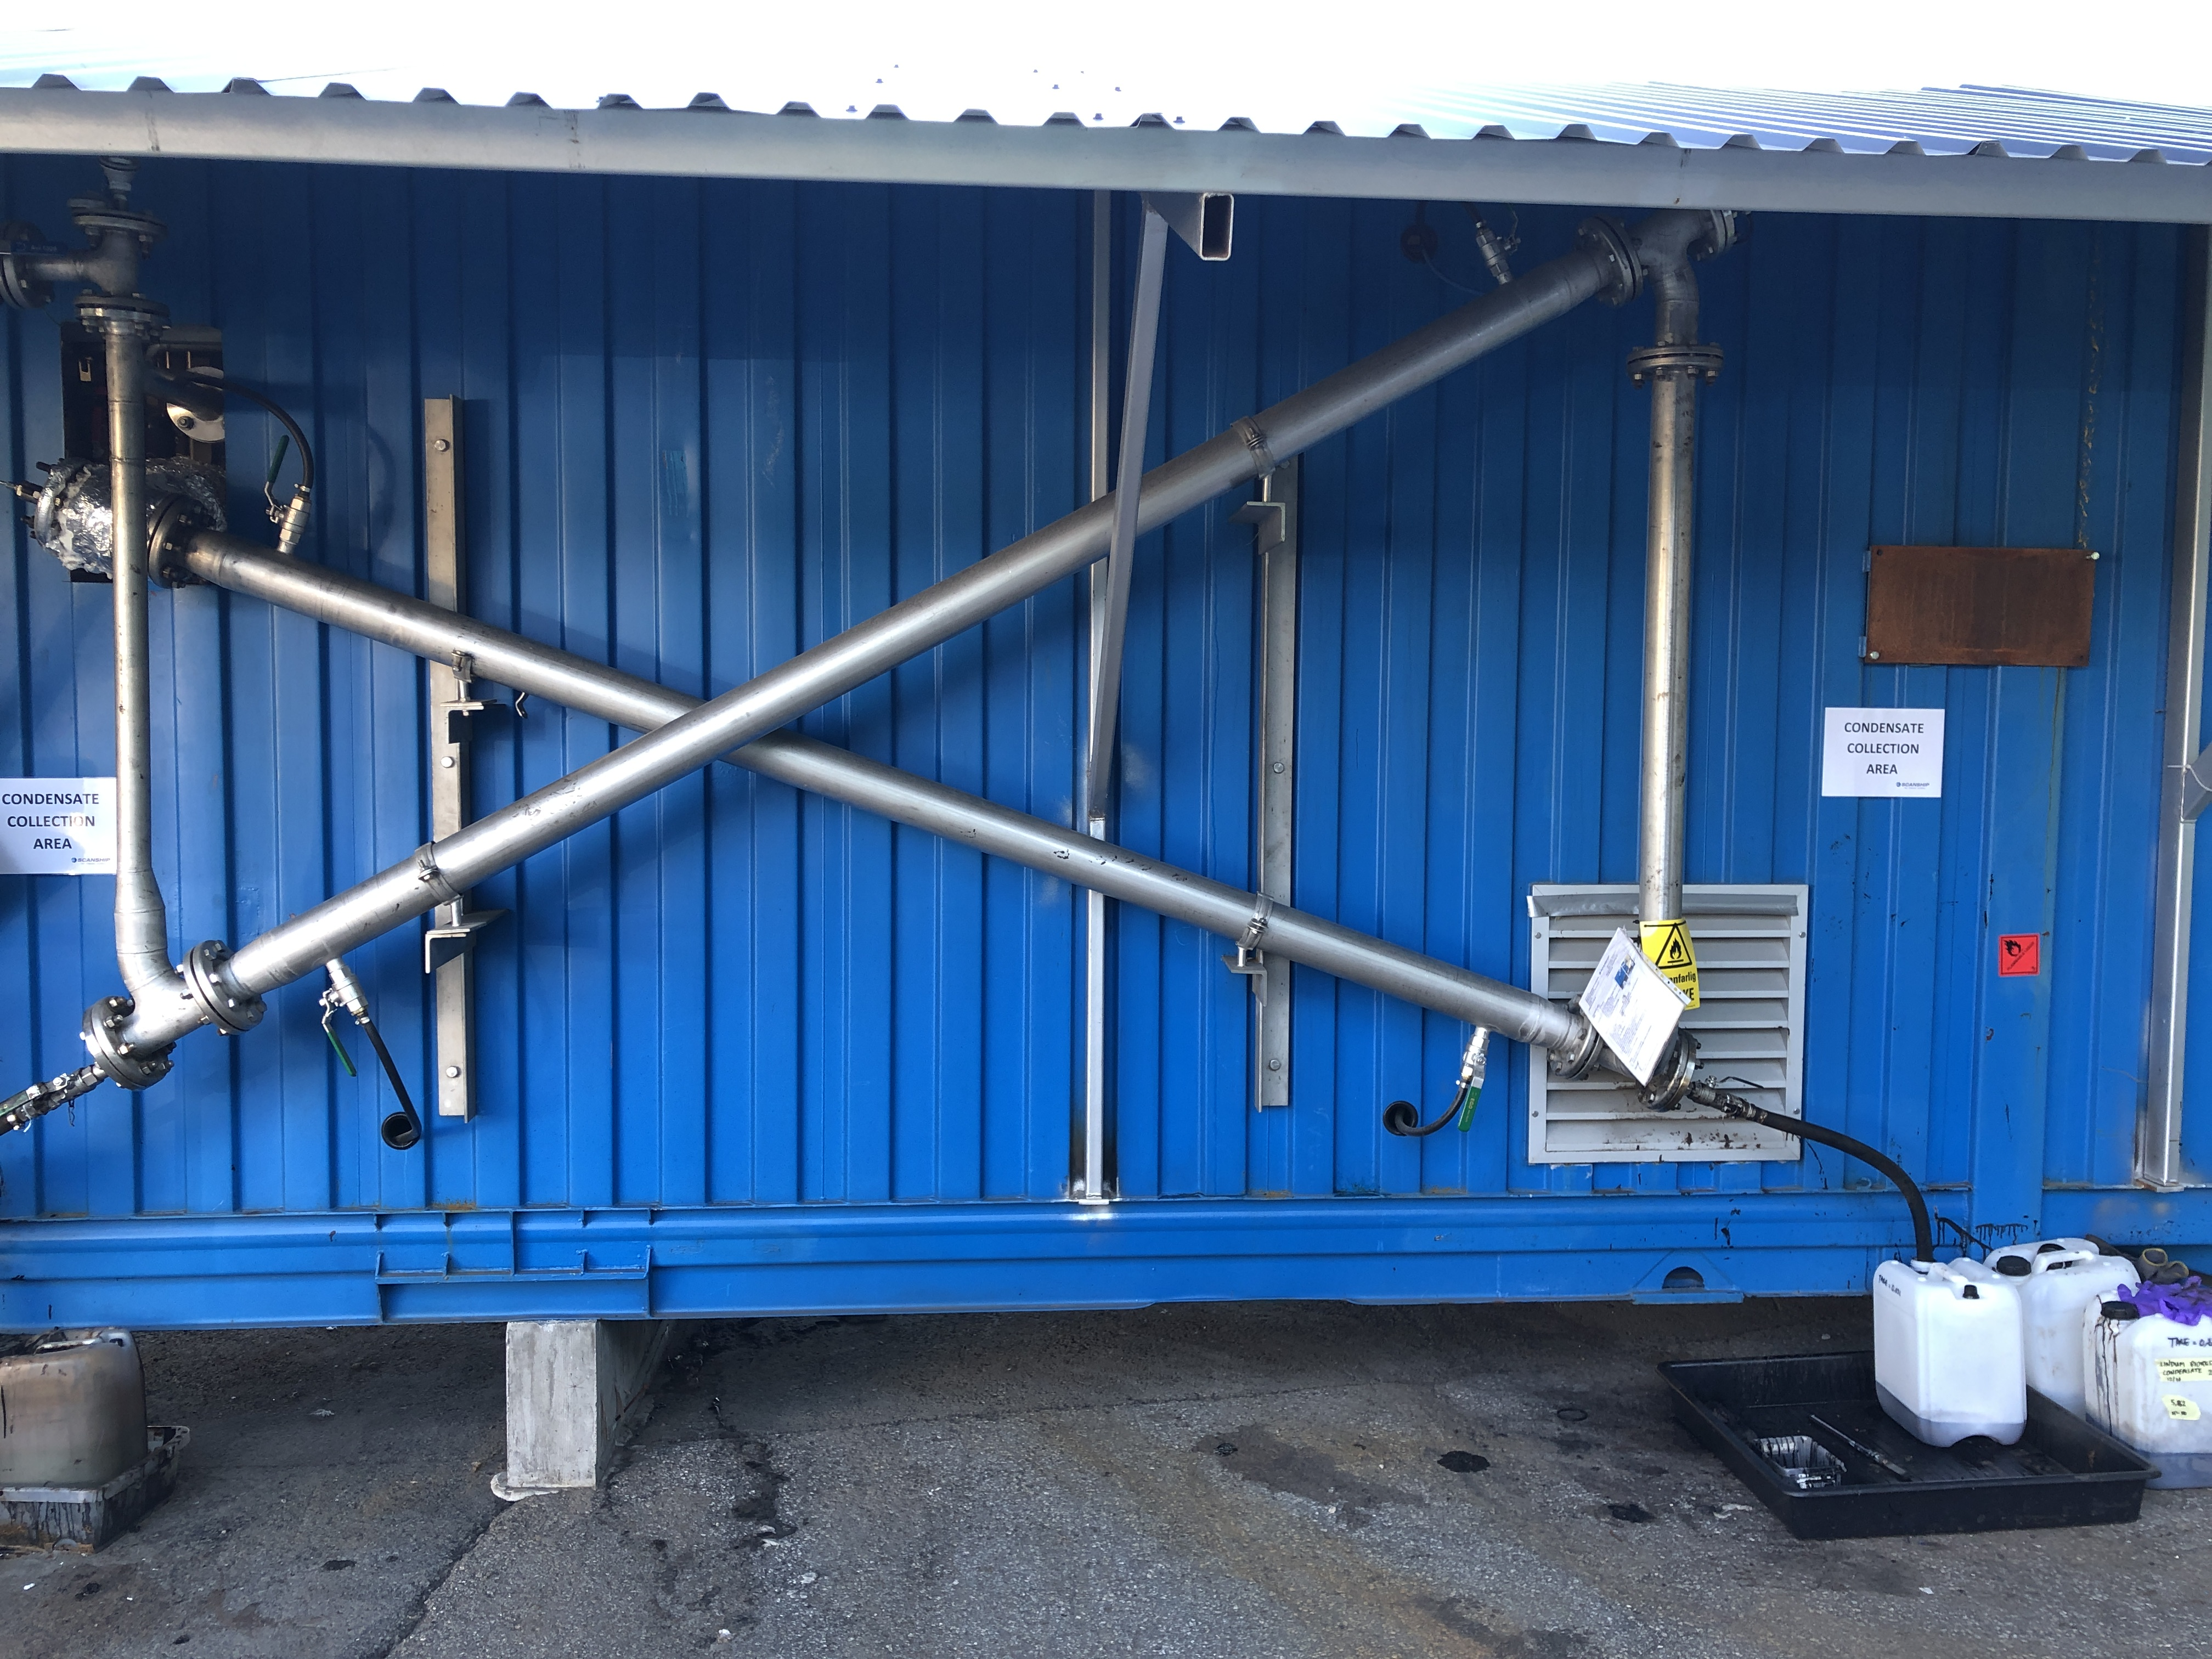
\includegraphics[width=0.6\linewidth,scale=0.6]{Bilder/Pyrolysis/Condenser.png}
         \hspace{0.5 cm}
         \caption{}
         \label{fig:condenserfull}
     \end{subfigure}
     \hfill
     \begin{subfigure}[b]{0.3\linewidth}
         \centering
         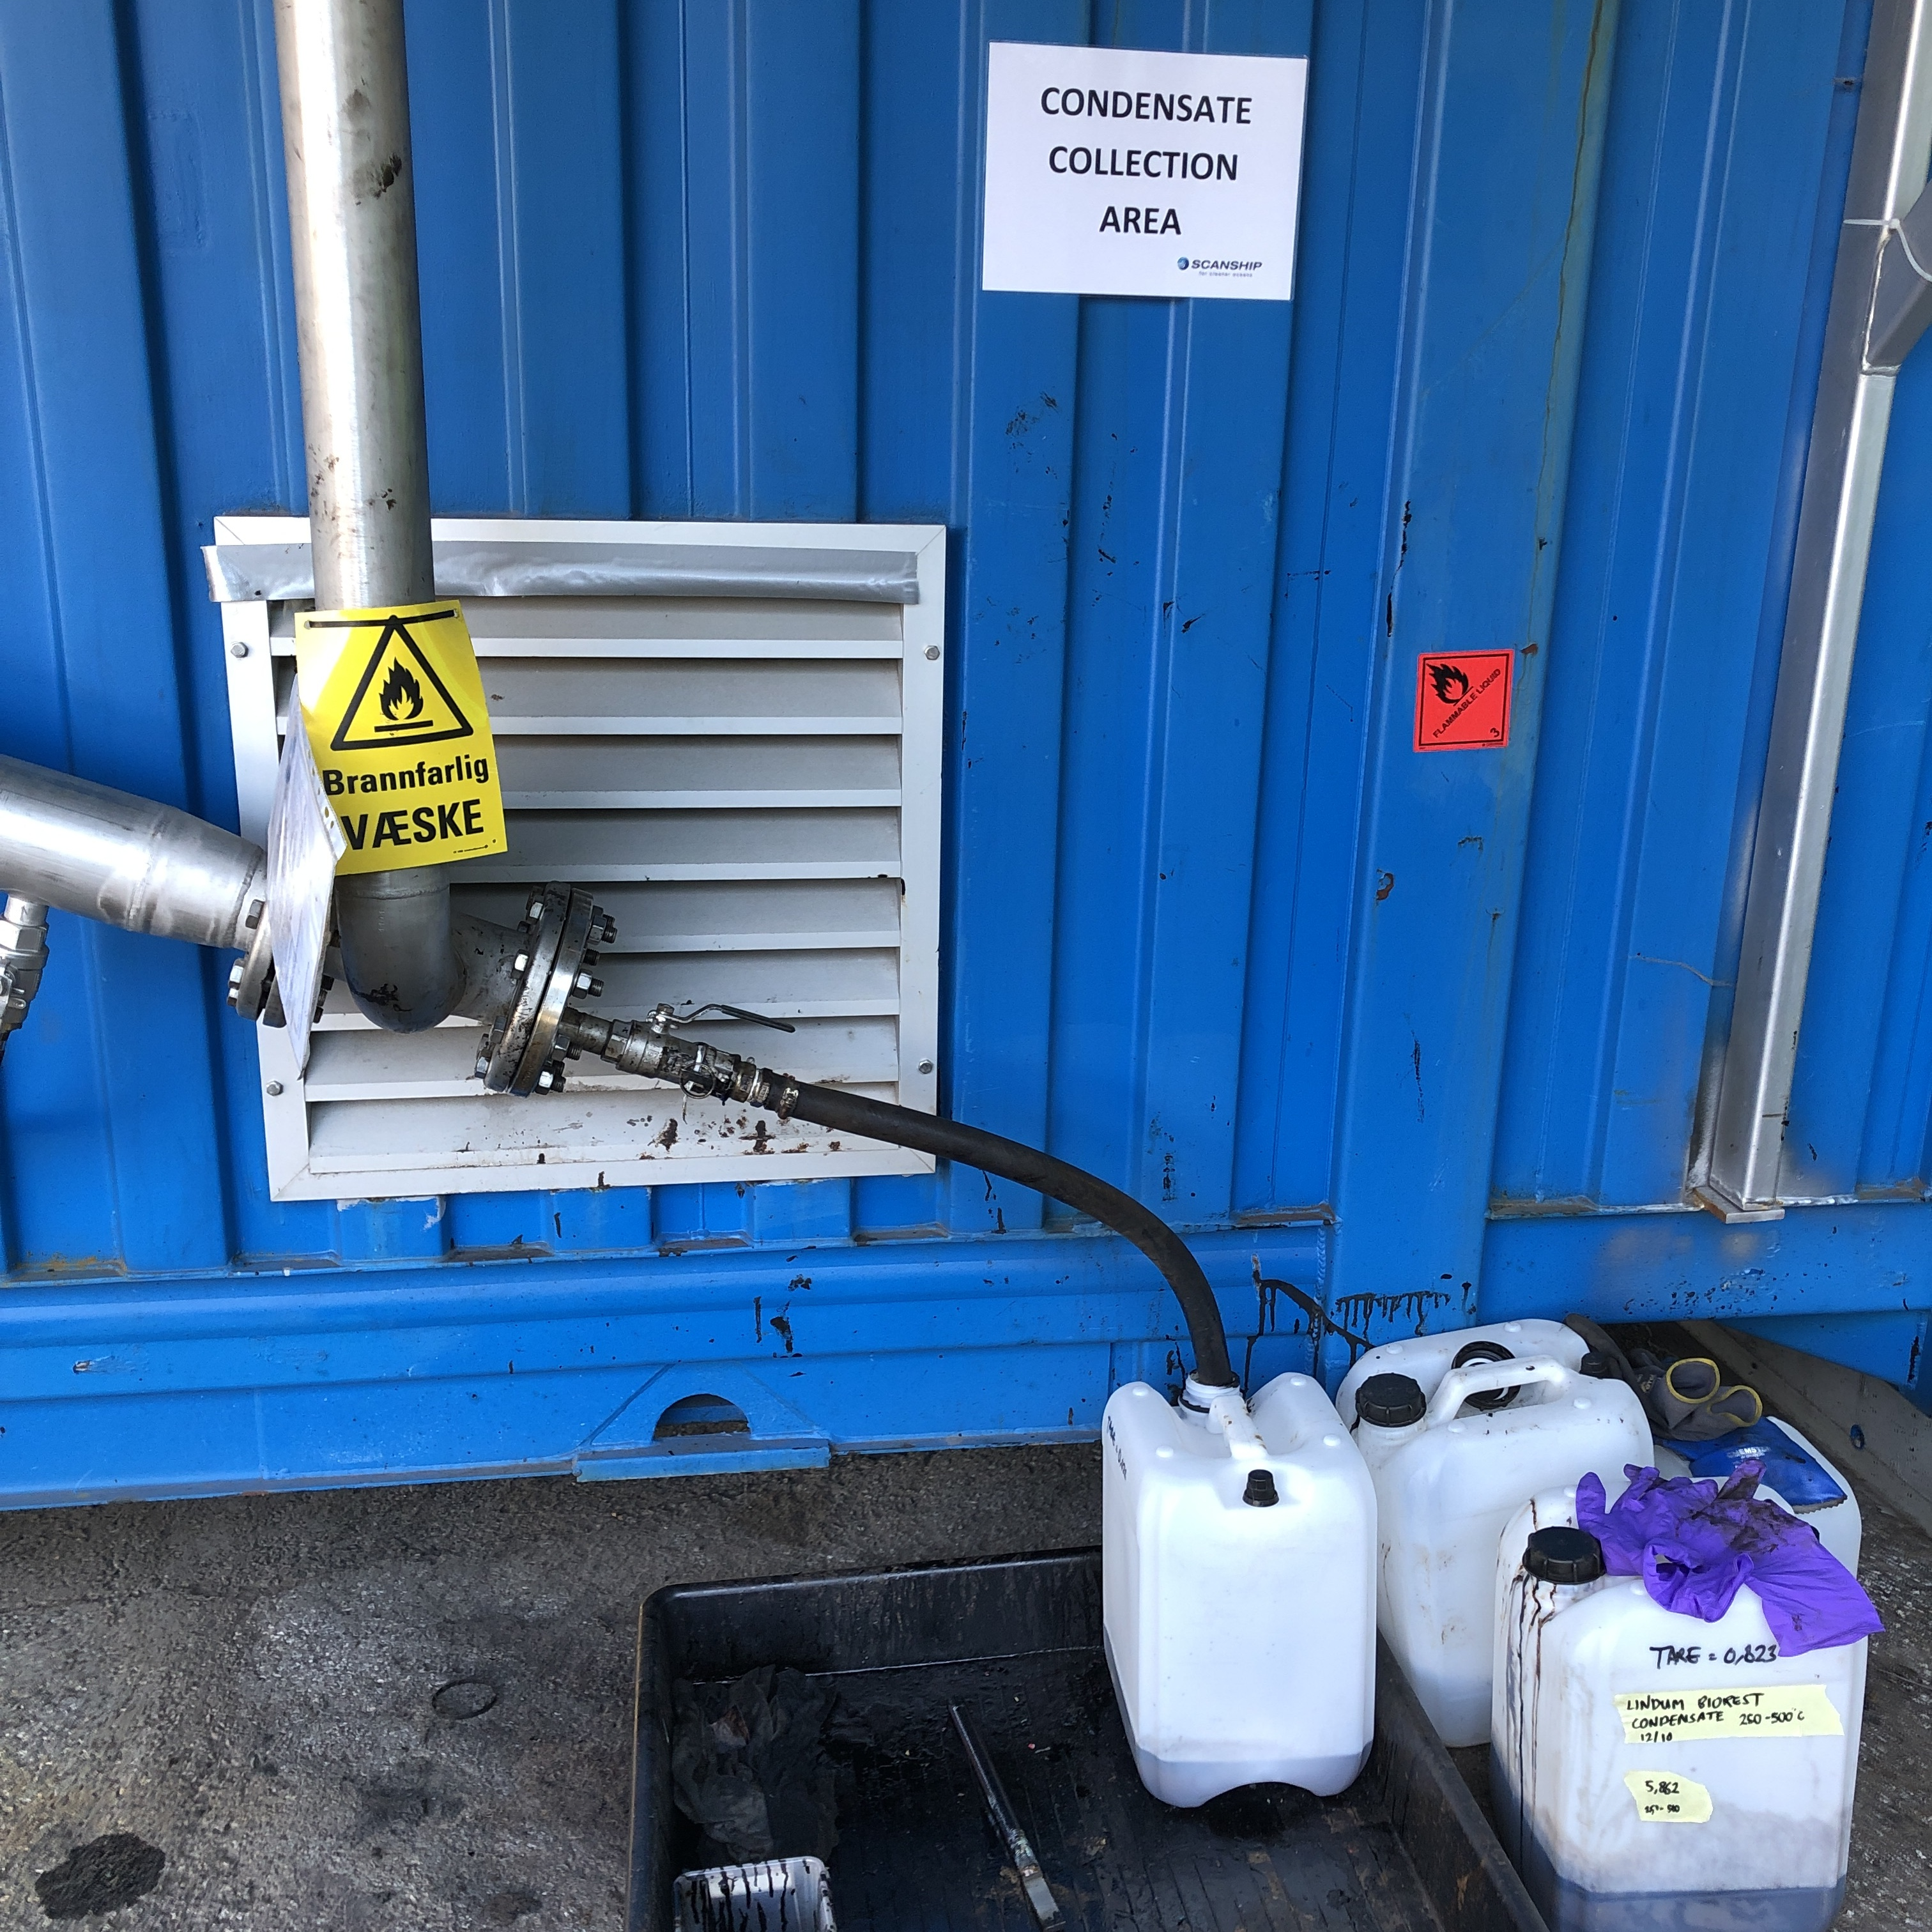
\includegraphics[width=\linewidth]{Bilder/Pyrolysis/CondensateCollection1.jpg}
         \caption{}
         \label{fig:condensate1}
     \end{subfigure}
     \hfill
     \begin{subfigure}[b]{0.3\linewidth}
         \centering
         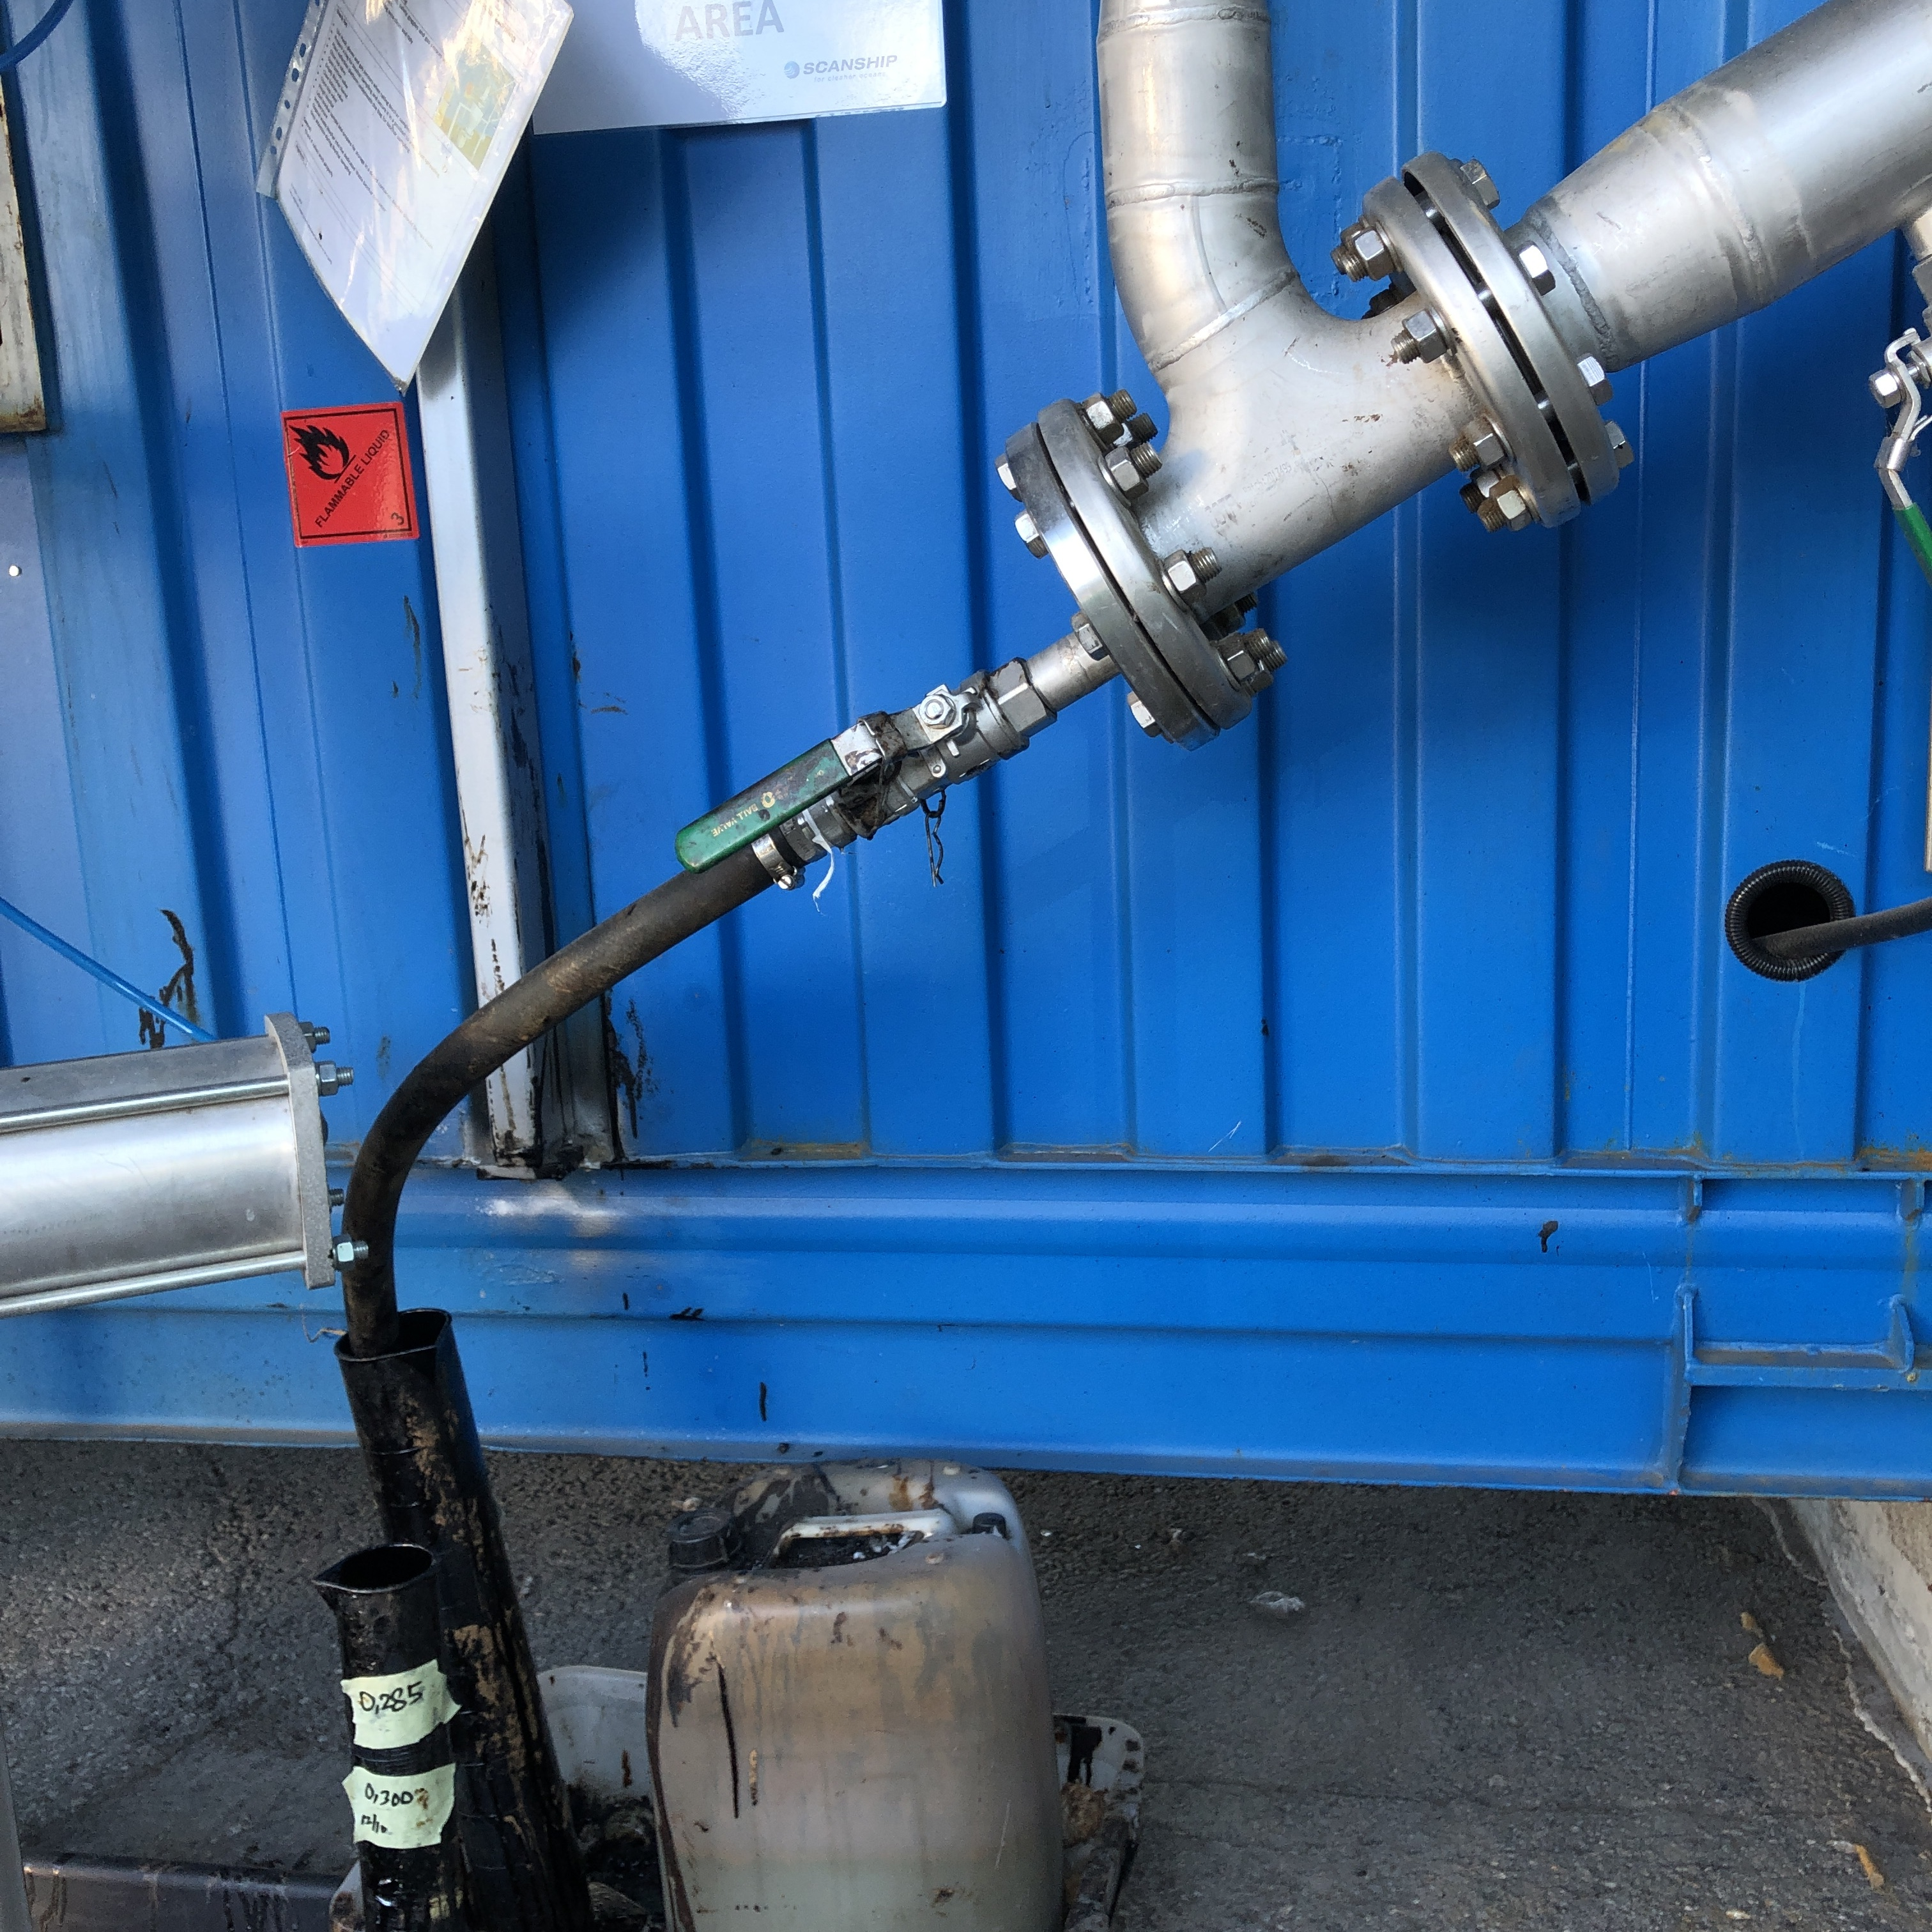
\includegraphics[width=\linewidth]{Bilder/Pyrolysis/CondensateCollection2.jpg}
         \caption{}
         \label{fig:condensate2}
     \end{subfigure}
        \caption{Syn-gas condenser. (a) First condensate collection area draining long-chain bio-oils. (b) Second condensate collection area draining short-chain bio-oils.}
        \label{fig:condenser}
\end{figure}

\begin{table}
    \centering
    \caption{Purity, stock form and LOQs of the PFCAs used for the sorption isotherms. iLOQ = instrumental LOQ for  the extract, mLOQ = method LOQ.}
    \label{tab:PFCAform&LOQ}
    \begin{tabular}{@{}lllccc@{}}
    \toprule
    \multicolumn{1}{l}{Compound}  & \multicolumn{1}{l}{Purity}  & \multicolumn{1}{l}{Stock form} & \multicolumn{1}{l}{iLOQ} & \multicolumn{1}{l}{mLOQ}  & \multicolumn{1}{l}{2$\times$mLOQ}\\ 
    & & & \multicolumn{1}{l}{(ng mL\textsuperscript{-1})}  & \multicolumn{1}{l}{(ng L\textsuperscript{-1})}  & \multicolumn{1}{l}{(ng L\textsuperscript{-1})} \\ \midrule
     PFPeA  & 97 \%   & liquid    & 0.05 & 0.50  & 1.00     \\
     PFHxA  & 97 \%   & liquid    & 0.10 & 1.00   & 2.00     \\
     PFHpA-K  & 99 \%   & crystalline & 0.01 & 0.10   & 0.20    \\
     PFOA-K   & 95 \%   & powder    & 0.05 & 0.50    & 1.00   \\
     PFNA-K   & 97 \%    & crystalline  & 0.05 & 0.50 & 1.00   \\
     PFDA-K   & 98 \% & flakes & 0.10 & 1.00 & 2.00  \\ \bottomrule
    \end{tabular}
\end{table}

 The cartridges used for extraction of PFAS  Strata\textsuperscript{\textregistered}-X Phenomenex: Cartridges with  200 mg/6mL 
 
 Gabi
 Determination of target analytes was performed in an UPLC-MS/MS with a Xevo TQ-S triple quadrupole mass spectrometer furnished with a ESI Z spray, and connected to an Acquity UPLC I-Class system, both acquired from Waters (Milford, MA, U.S.). Chromatographic separation was carried out in a Kinetex C18 column (30 x 2.1 mm, 1.3 μm) serially connected to a C18 (2 x 2.1 mm i.d.) security guard, both supplied by Phenomenex (Torrance, CA, U.S.). Milli-Q water 2 mM ammonium acetate (A) and pure MeOH (B), were used as mobile phases at a constant flow rate of 250 μL min-1. The UPLC column and precolumn were maintained at 30 ºC. The mobile phase gradient was programmed as follows: 0-0.2 min, 10\% B; 3.0-3.5 min, 100\% B; 3.6-5 min, 10\% B. The injection volume was 4 μL. Analytes were ionized under negative ionization mode (ESI-). Nitrogen was used as drying gas at the ionization source (450ºC at 650 L hour-1). The capillary voltage was maintained at 2 kV, the cone voltage at 25 V, and the source offset voltage at 40 V. Two transitions were monitored per chemical (Table 1) considering a time window of 60 s around their retention time. The dwell time per transition was automatically adjusted by the MassLynx software to obtain 12 points per peak assuming an average baseline peak width of 5 s. 
UPLC-MS/MS data was acquired with MassLynx version 4.1 software, while quantification processing was performed with TargetLynx (Waters, Milford, U.S.).

Procedural blank: IS spiked directly into cartridge and eluted with methanol to check contamination during the extraction protocol. If the reagent blank is contaminated, the signal must be subtracted from the rest of the samples. 
Three matrix matched samples with the same concentrations as the pre-extraction spikes that were submitted to the entire protocol where the addition of IS and analytes were made post-extraction, just to calculate recoveries \cref{eq:Recovery,eq:ME}.
Gabi:
%Contamination arising from sampling and laboratory materials was evaluated through the analysis of sampling and procedural blanks. Working benches were cleaned with acetone and covered with aluminum foil before sample preparation. In addition, clean PP material was used during the complete protocol. During analysis, solvent blanks, and a mixture of standards of 10 ng mL-1 were injected every 15 injections along the sequence to check for any potential cross contamination or sample carryover, and to evaluate signal variations and potential drifting time. A solution of MeOH:Milli-Q (50:50; v/v) 0.1 \% formic acid was used as wash solution for cleaning the injection needle during 8 and 10 seconds before and after each injection.

%A 10-point calibration curve with concentrations ranging from 0.01 to 20.0 ng mL-1 (0.01, 0.05, 0.10, 0.20, 0.50, 1.00, 2.00, 5.00, 10.0, and 20.0 ng mL-1) was prepared, and demonstrated a satisfactory regression coefficient for every target analyte (R2 > 0.98). Pre- and post- extraction spiked matrix samples were used as QA/QC samples and were prepared by spiking known amounts of the target analytes and internal standards prior and post to the sample preparation, respectively. The extraction recoveries of the method were assessed in pooled matrix at three different amounts (2.5, 5, 10 ng mL-1; n=3 replicates per amount). Matrix effects (MEs, \%) during measurements were assessed and estimated as XXXX. Quantification of the target analytes was accomplished based on the internal standard method and with matrix-matched calibration standards.

%Contamination arising from sampling and laboratory materials was evaluated through the analysis of sampling and procedural blanks. Working benches were cleaned with acetone and covered with aluminum foil before sample preparation. In addition, clean PP material was used during the complete protocol. During analysis, solvent blanks, and a mixture of standards of 10 ng mL-1 were injected every 15 injections along the sequence to check for any potential cross contamination or sample carryover, and to evaluate signal variations and potential drifting time. A solution of MeOH:Milli-Q (50:50; v/v) 0.1 \% formic acid was used as wash solution for cleaning the injection needle during 8 and 10 seconds before and after each injection.

%A 10-point calibration curve with concentrations ranging from 0.01 to 20.0 ng mL-1 (0.01, 0.05, 0.10, 0.20, 0.50, 1.00, 2.00, 5.00, 10.0, and 20.0 ng mL-1) was prepared, and demonstrated a satisfactory regression coefficient for every target analyte (R2 > 0.98). Pre- and post- extraction spiked matrix samples were used as QA/QC samples and were prepared by spiking known amounts of the target analytes and internal standards prior and post to the sample preparation, respectively. The extraction recoveries of the method were assessed in pooled matrix at three different amounts (2.5, 5, 10 ng mL-1; n=3 replicates per amount). Matrix effects (MEs, \%) during measurements were assessed and estimated as XXXX. Quantification of the target analytes was accomplished based on the internal standard method and with matrix-matched calibration standards.


\begin{figure}
    \centering
    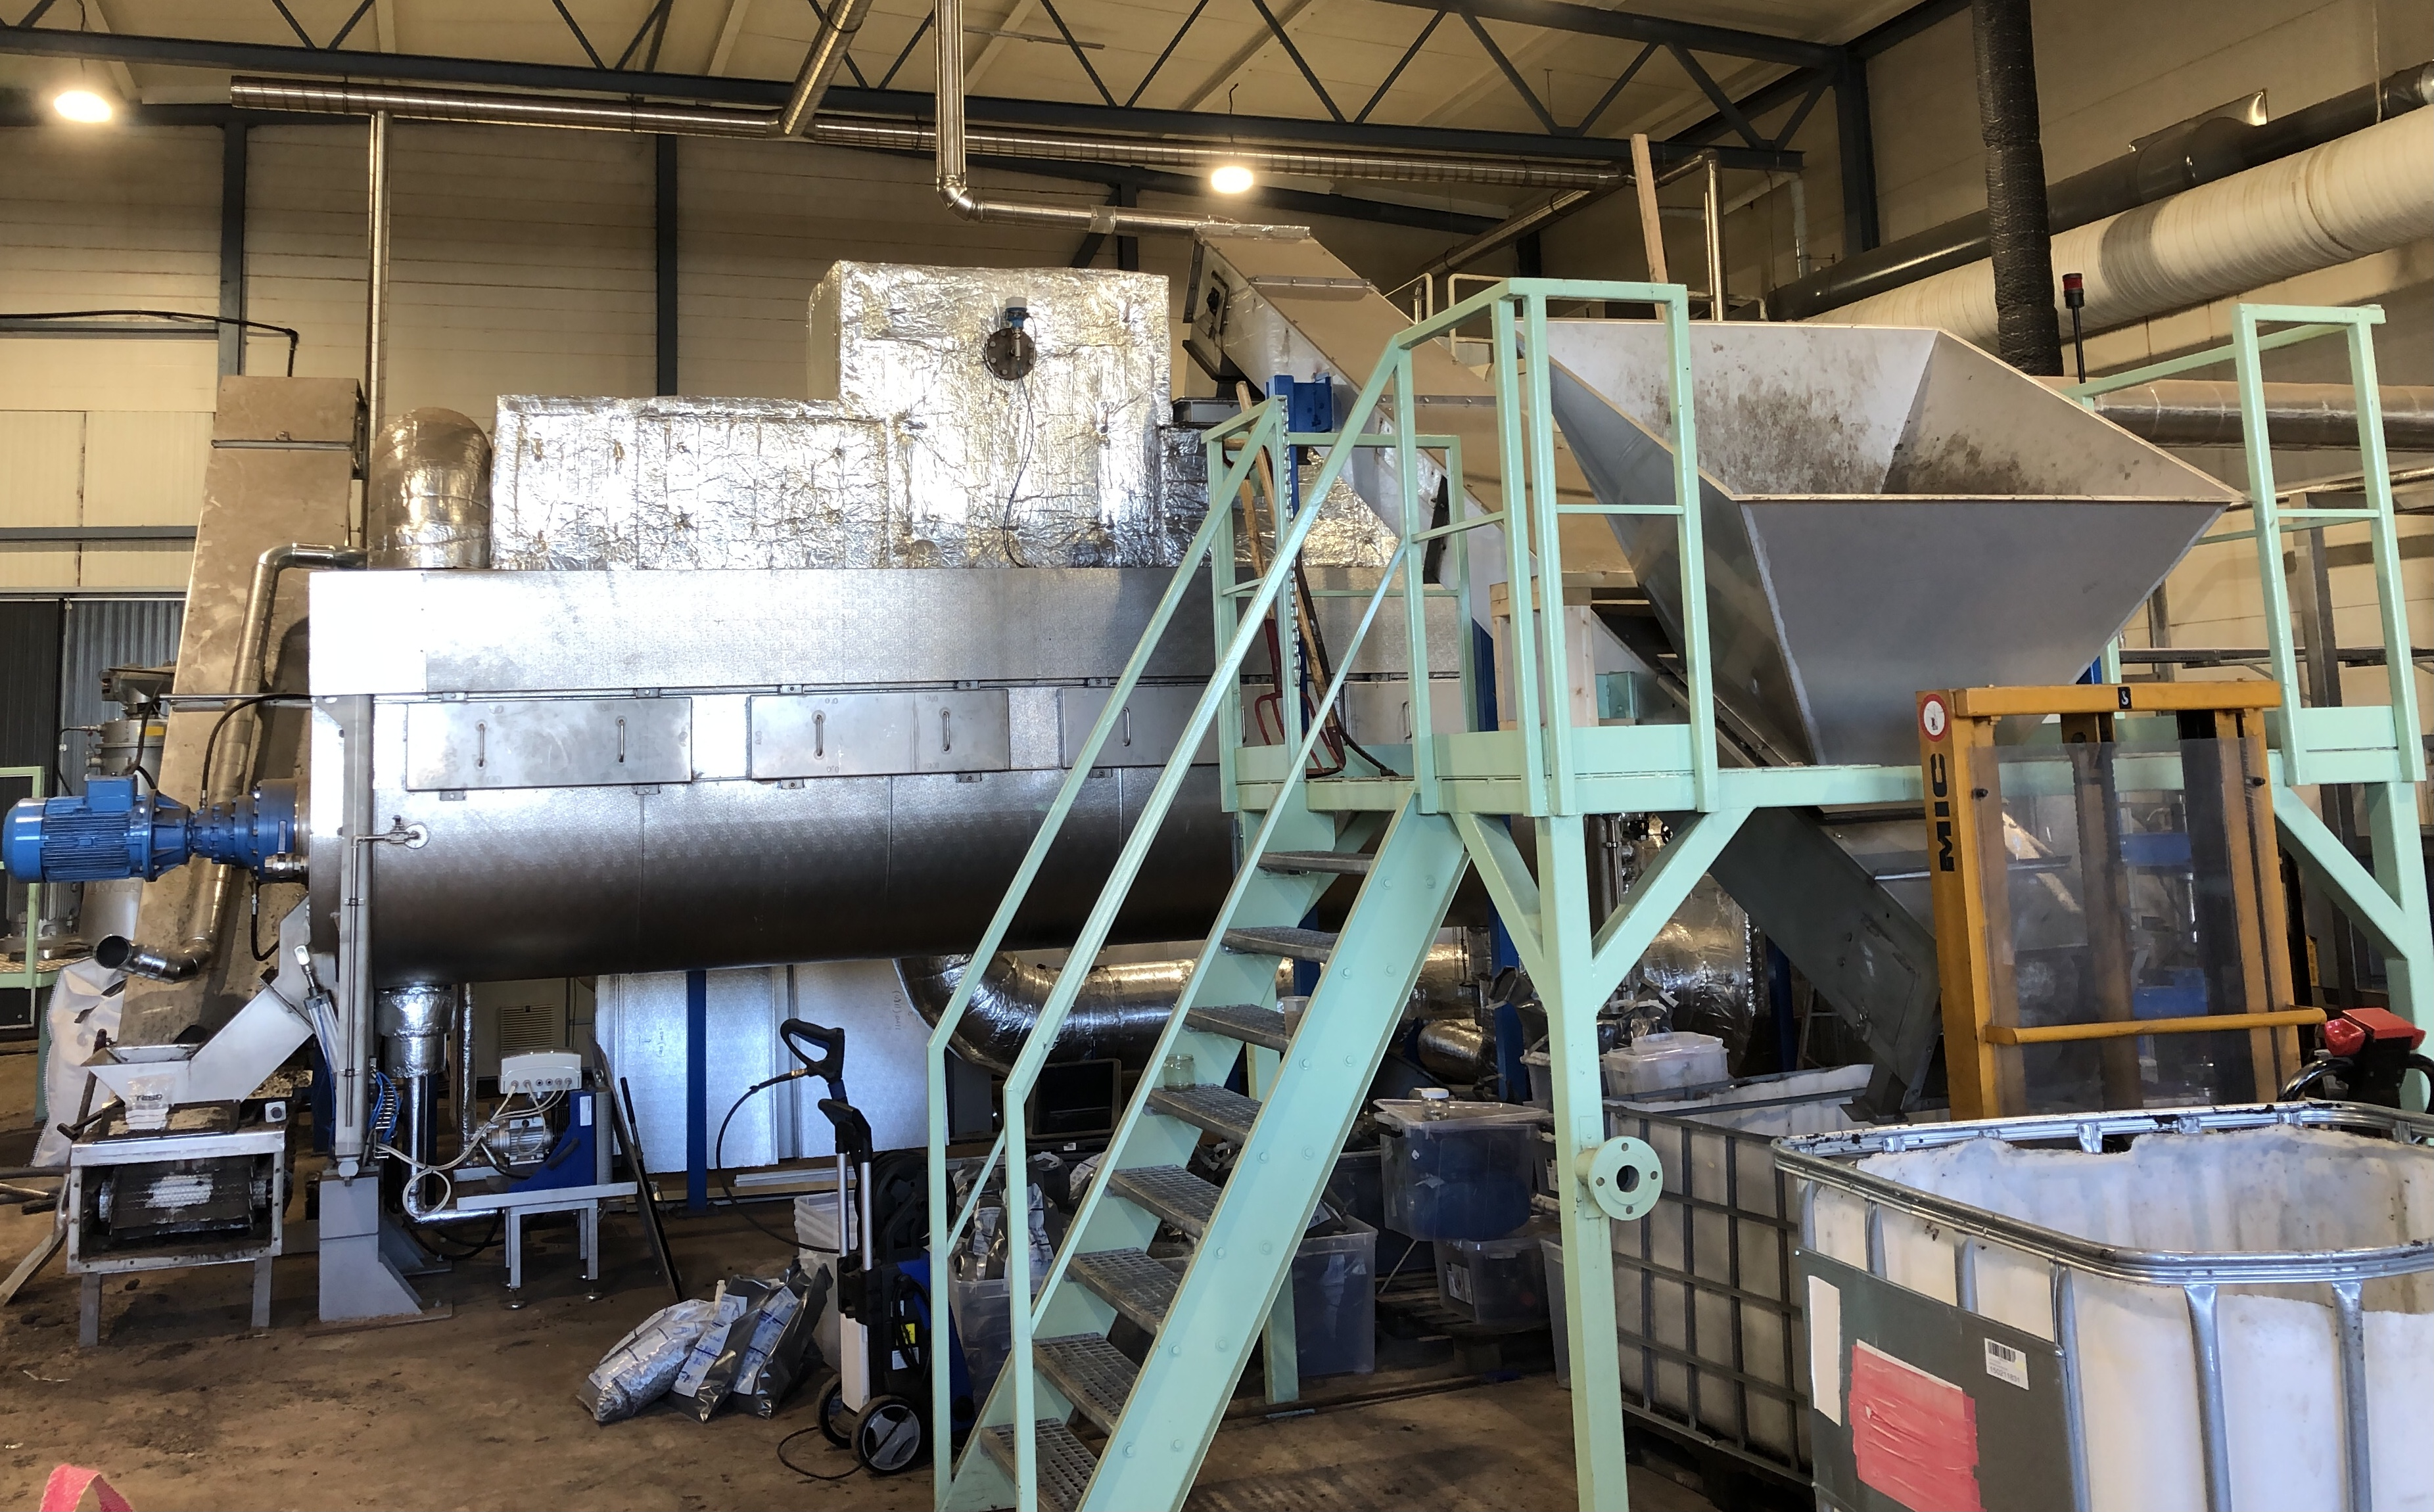
\includegraphics[width=0.7\linewidth,scale=0.7]{Bilder/Pyrolysis/Dryer.jpg}
    \caption{Sludge dryer at Lindum.}
    \label{fig:dryer}
\end{figure}

Biochar property characterization were performed at University of Florida, Gainsville\footnote{FL 32611, USA}. Iron and copper speciation was determined by XAS at the ESRF synchrotron (Grenoble, France).

\begin{figure}
    \centering
    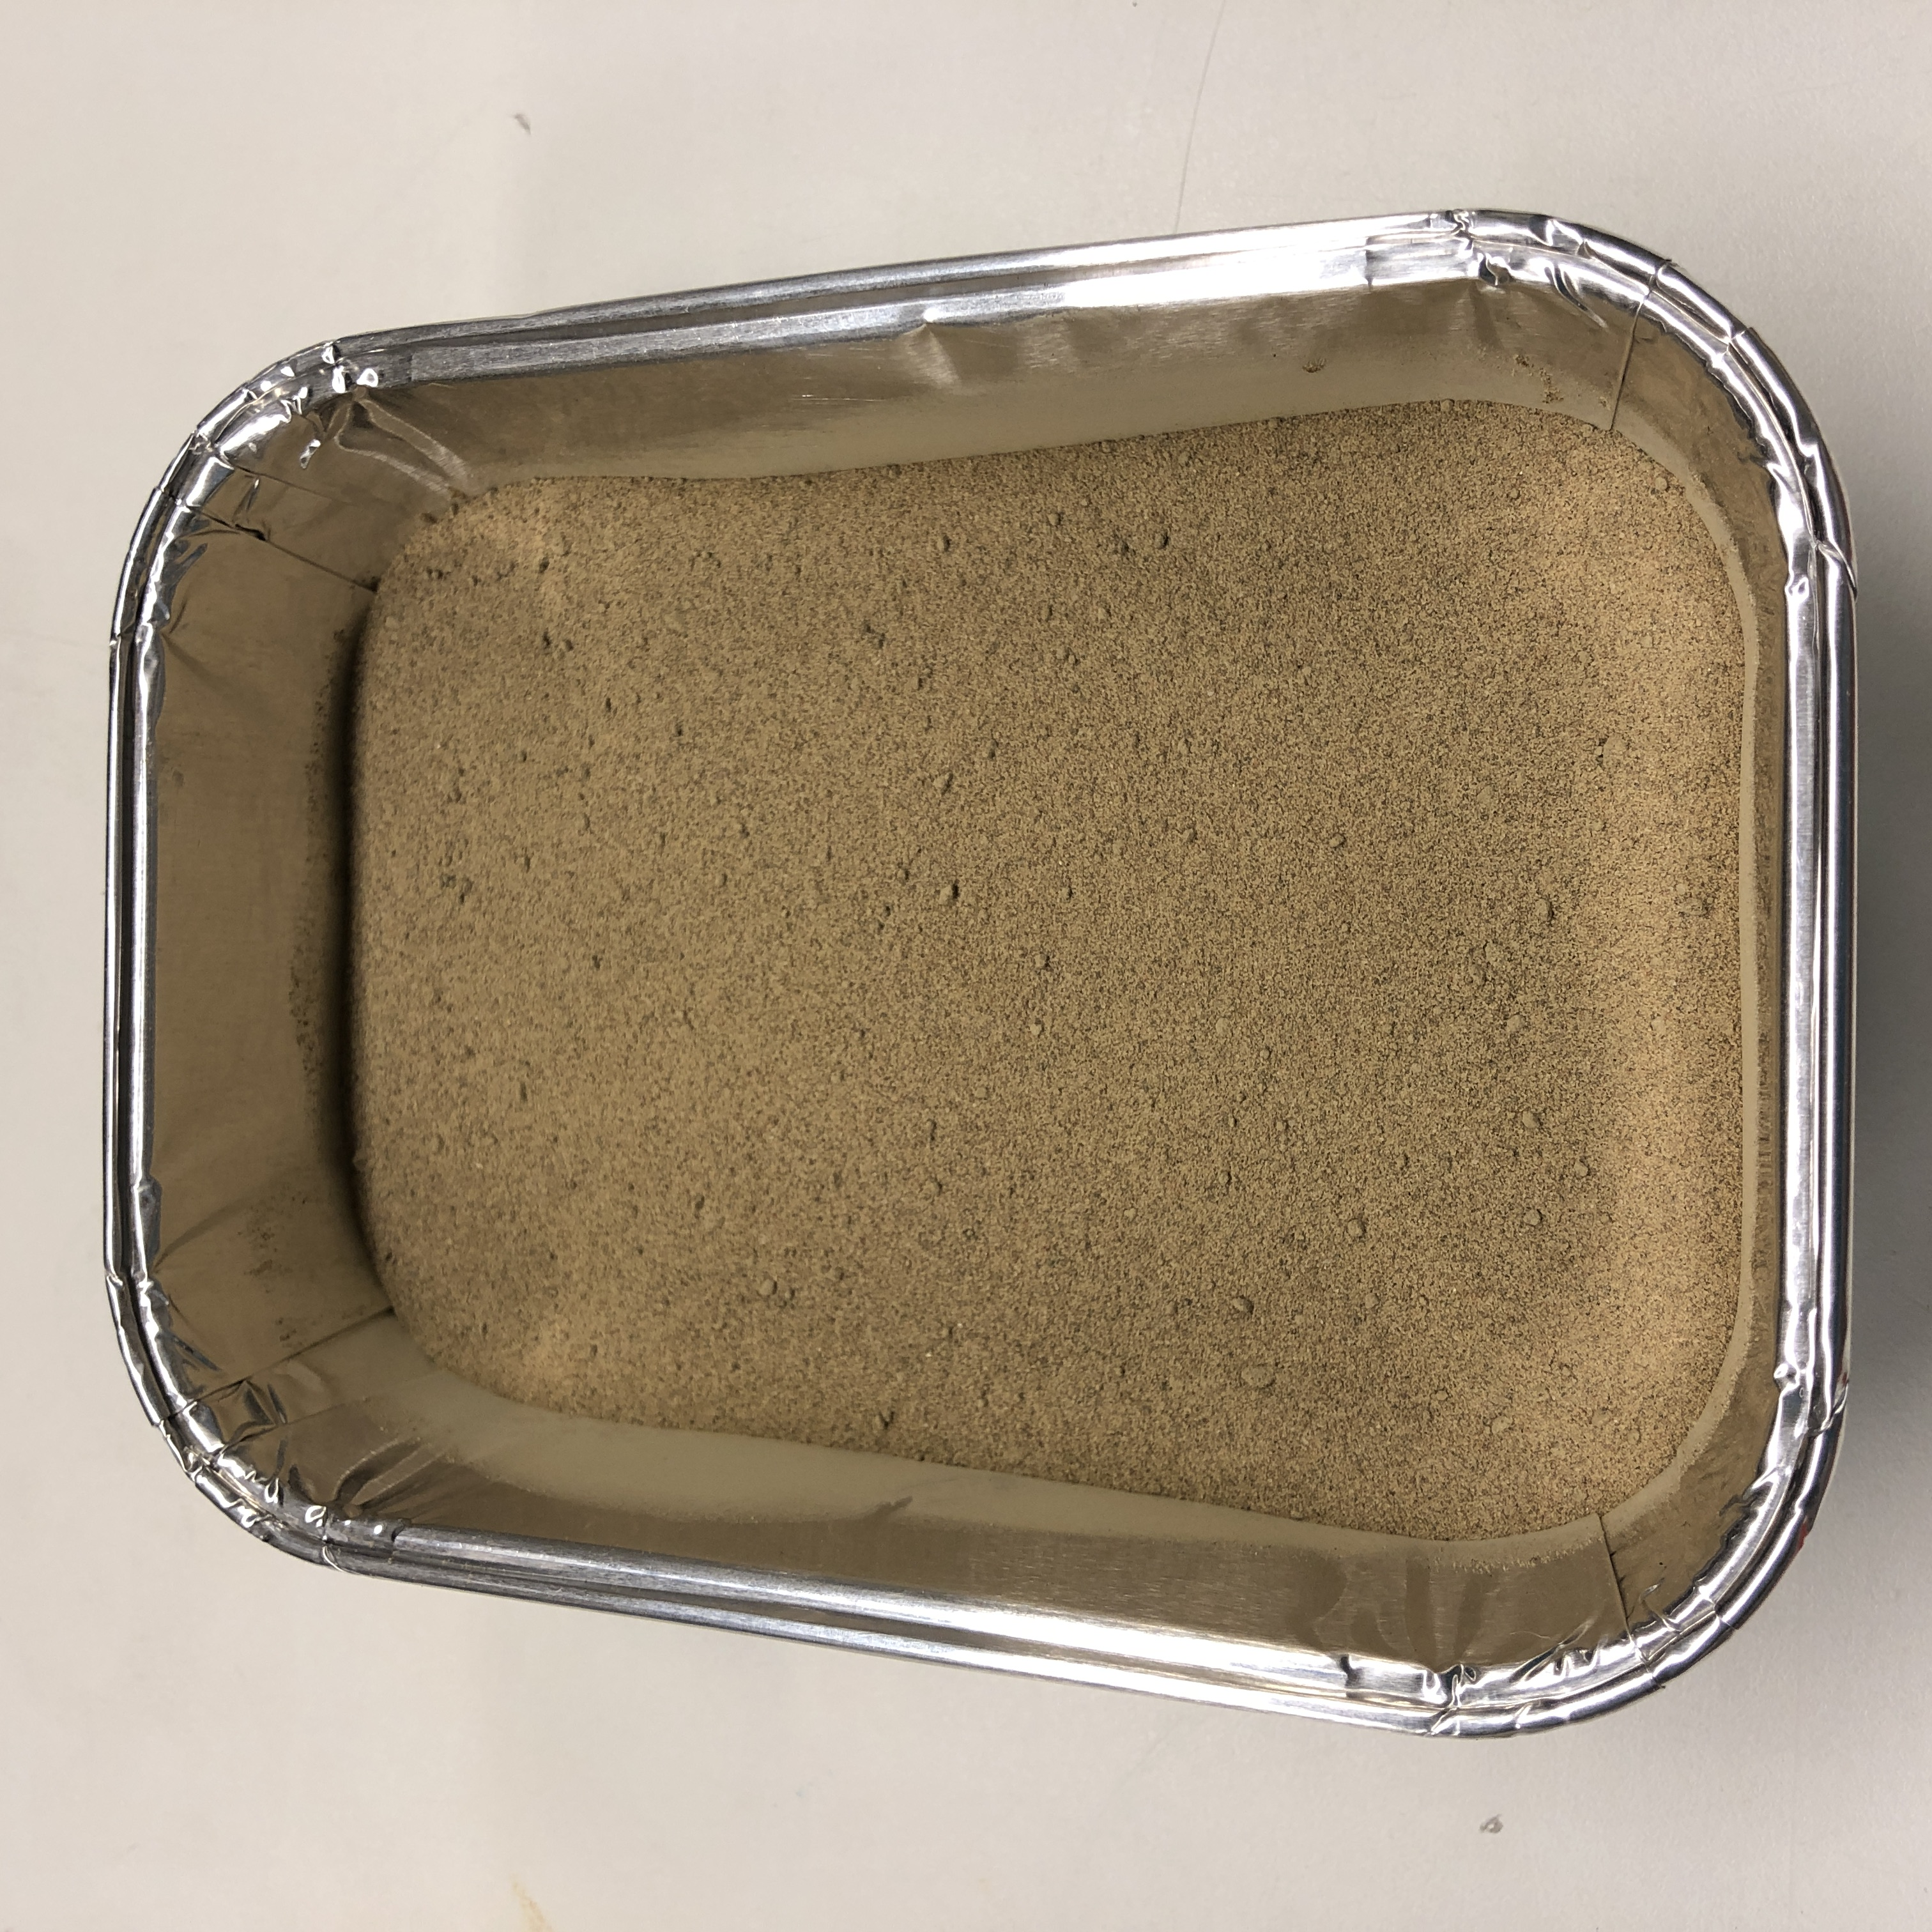
\includegraphics[width=0.5\textwidth]{Bilder/Samples/Soil_blank.JPG}
    \caption{The soil used for the batch tests.}
    \label{fig:soil}
\end{figure}

\begin{figure}
        \centering
         \begin{subfigure}[t]{\linewidth}
         \centering
         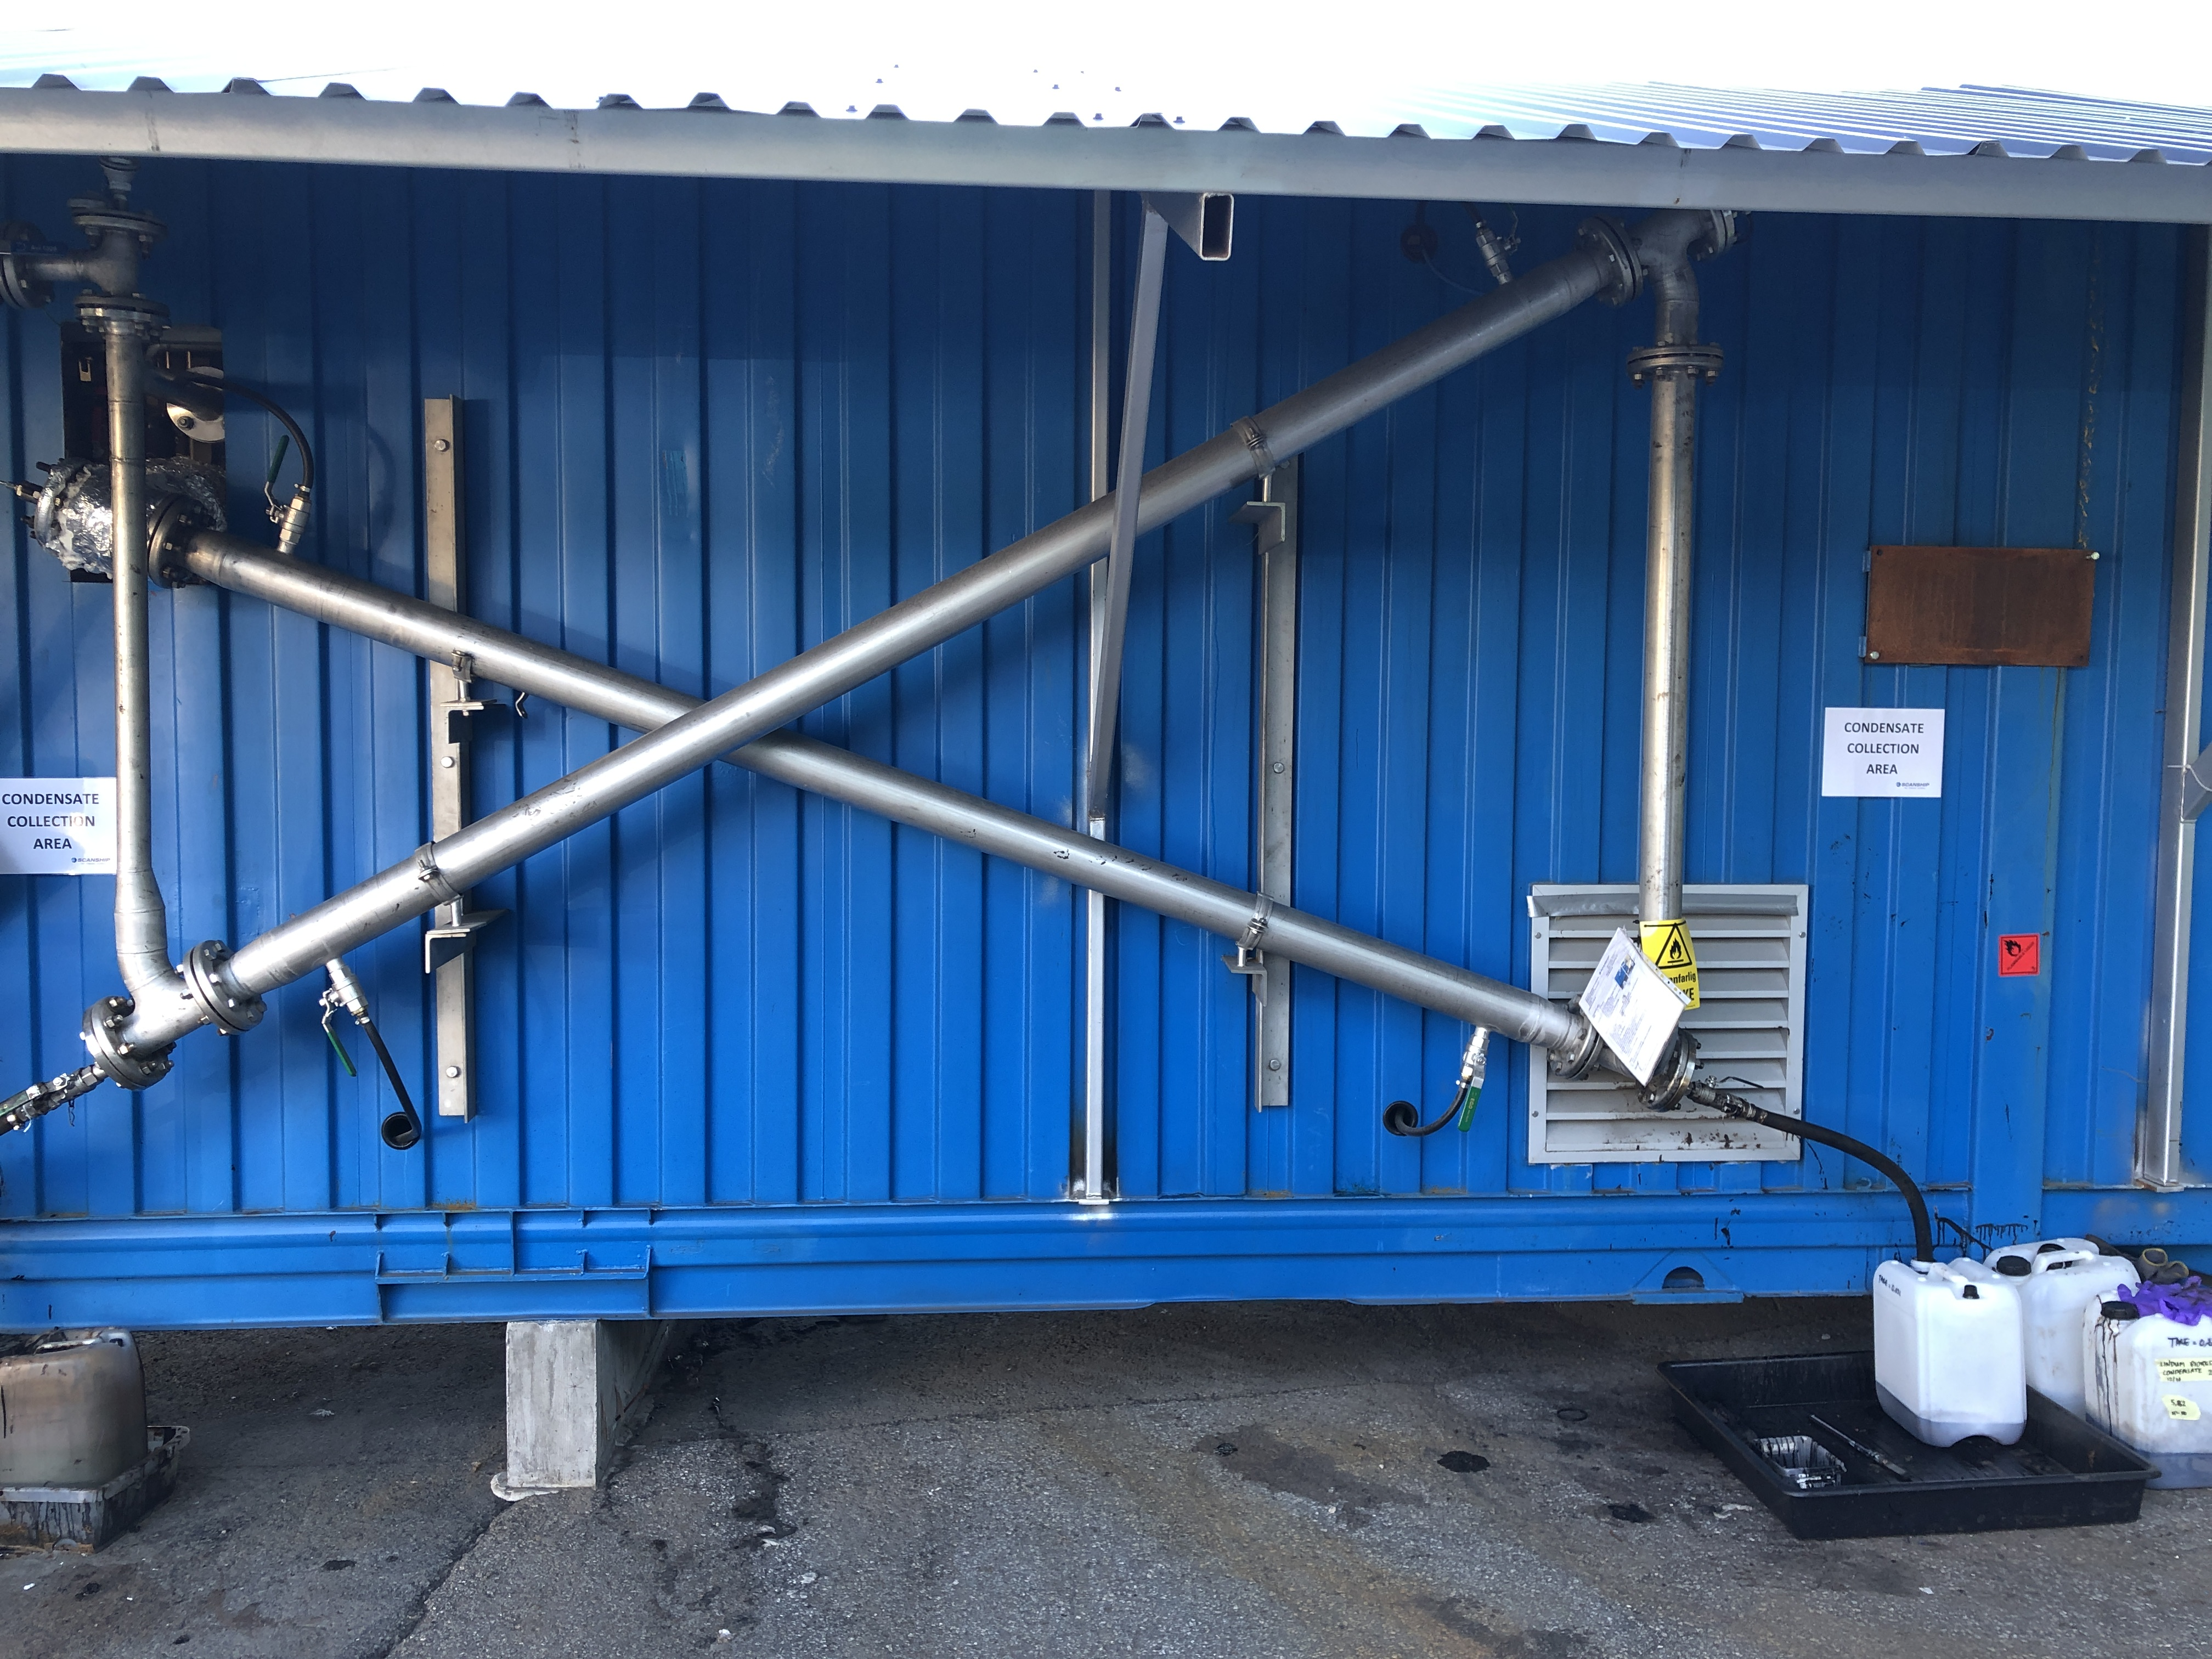
\includegraphics[width=0.74\linewidth,scale=0.74]{Bilder/Pyrolysis/Condenser.png}
         \caption{}
         \label{fig:condenserfull}
     \end{subfigure}
           \subfloat[]{%
              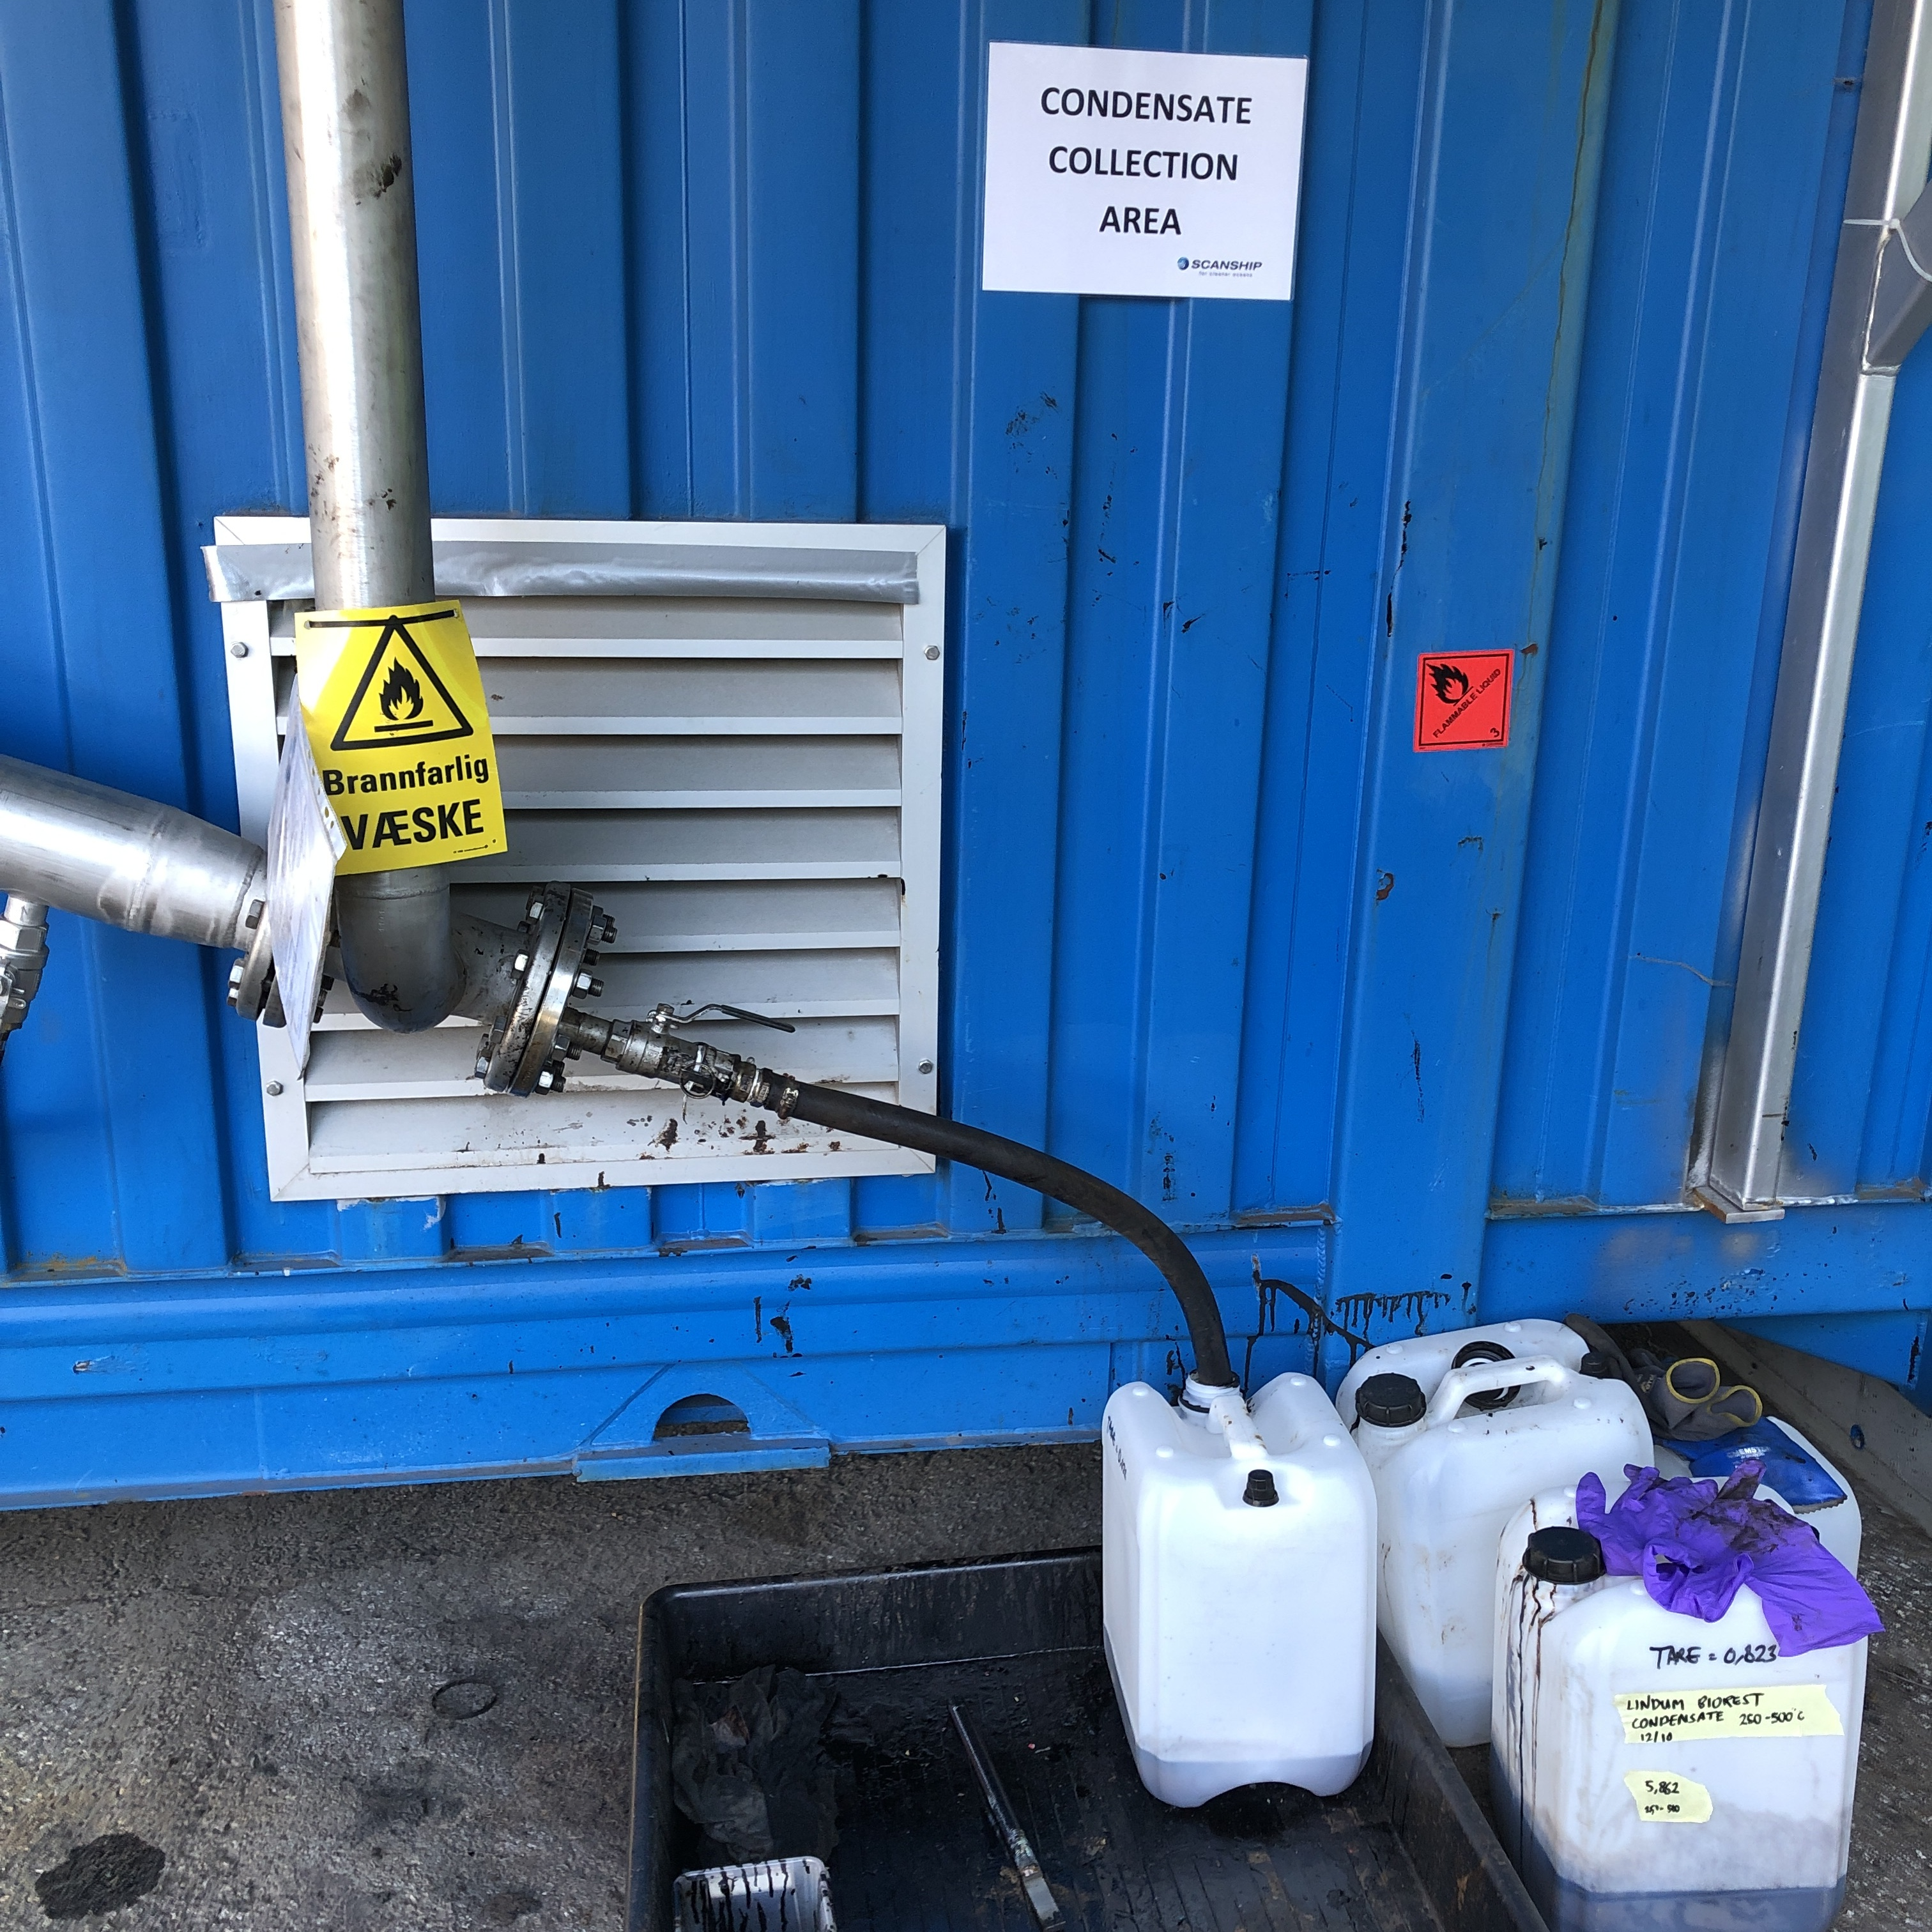
\includegraphics[height=6cm]{Bilder/Pyrolysis/CondensateCollection1.jpg}%
           }
           \hspace{0.5cm}
           \subfloat[]{%
              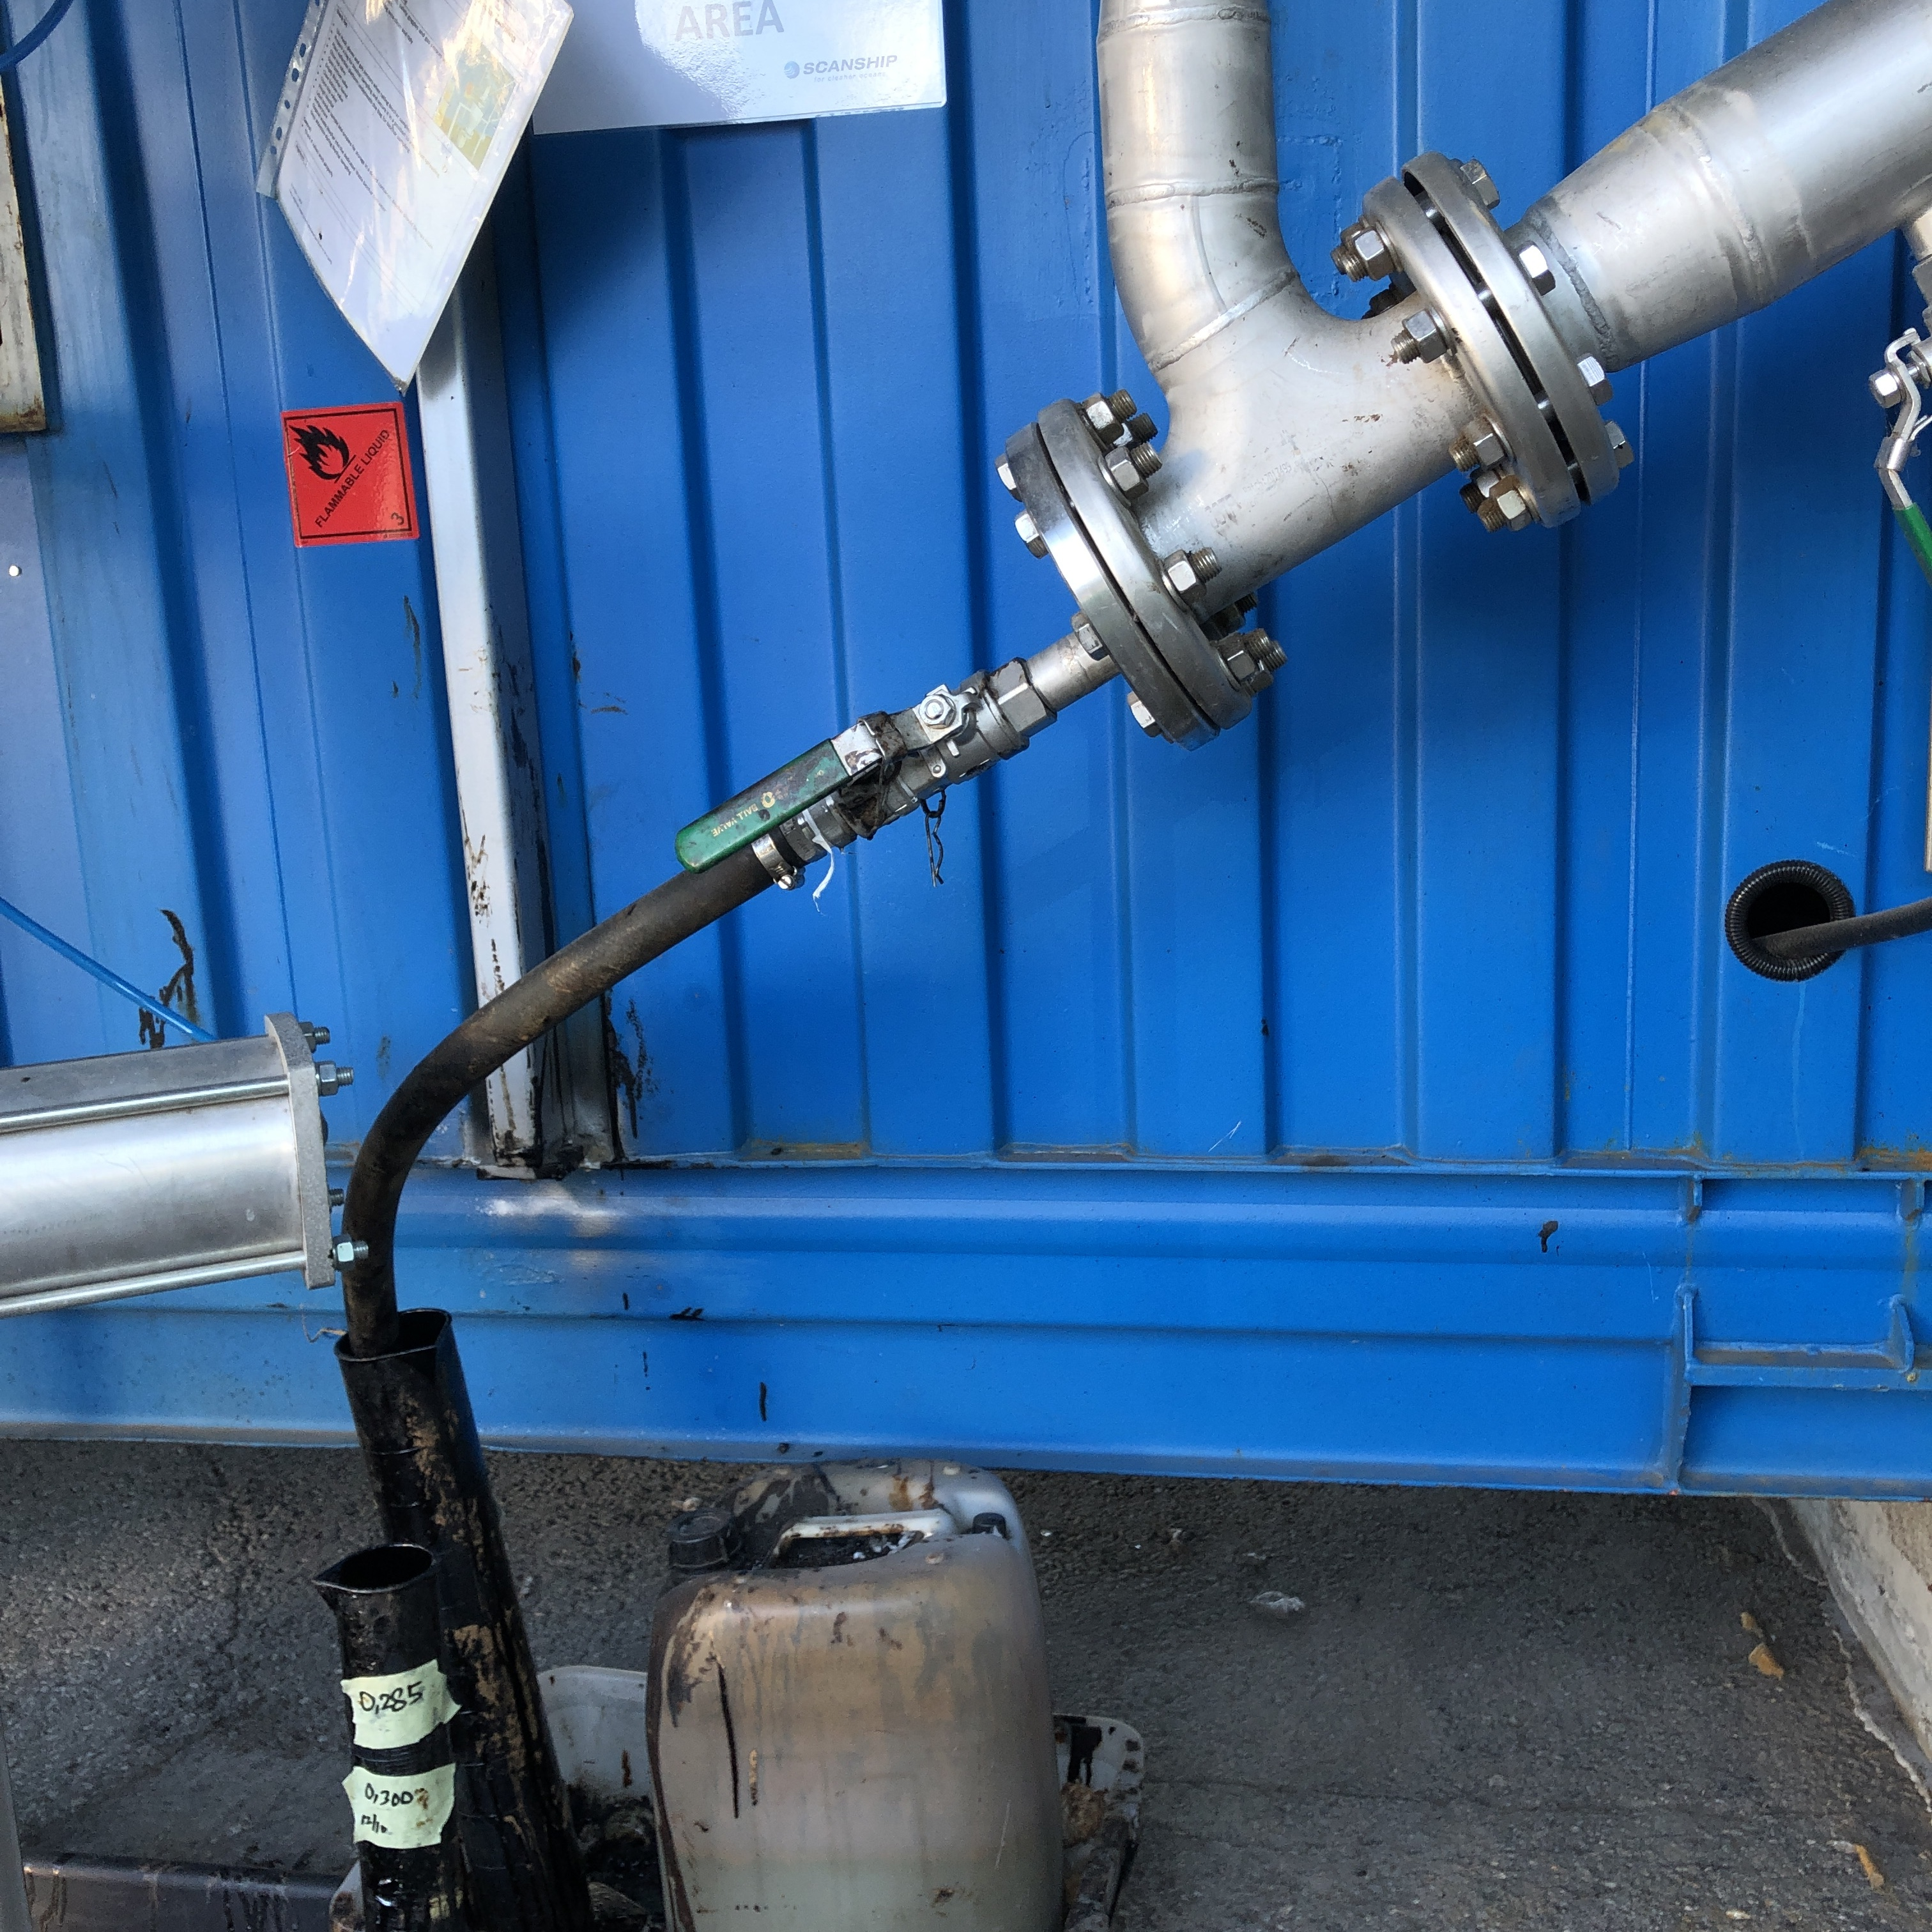
\includegraphics[height=6cm]{Bilder/Pyrolysis/CondensateCollection2.jpg}%
           }
        \caption{Syn-gas condenser. (a) First condensate collection area draining long-chain bio-oils. (b) Second condensate collection area draining short-chain bio-oils.}
        \label{fig:condenser}
\end{figure}

%consider omitting this figure
\begin{figure}
    \centering
    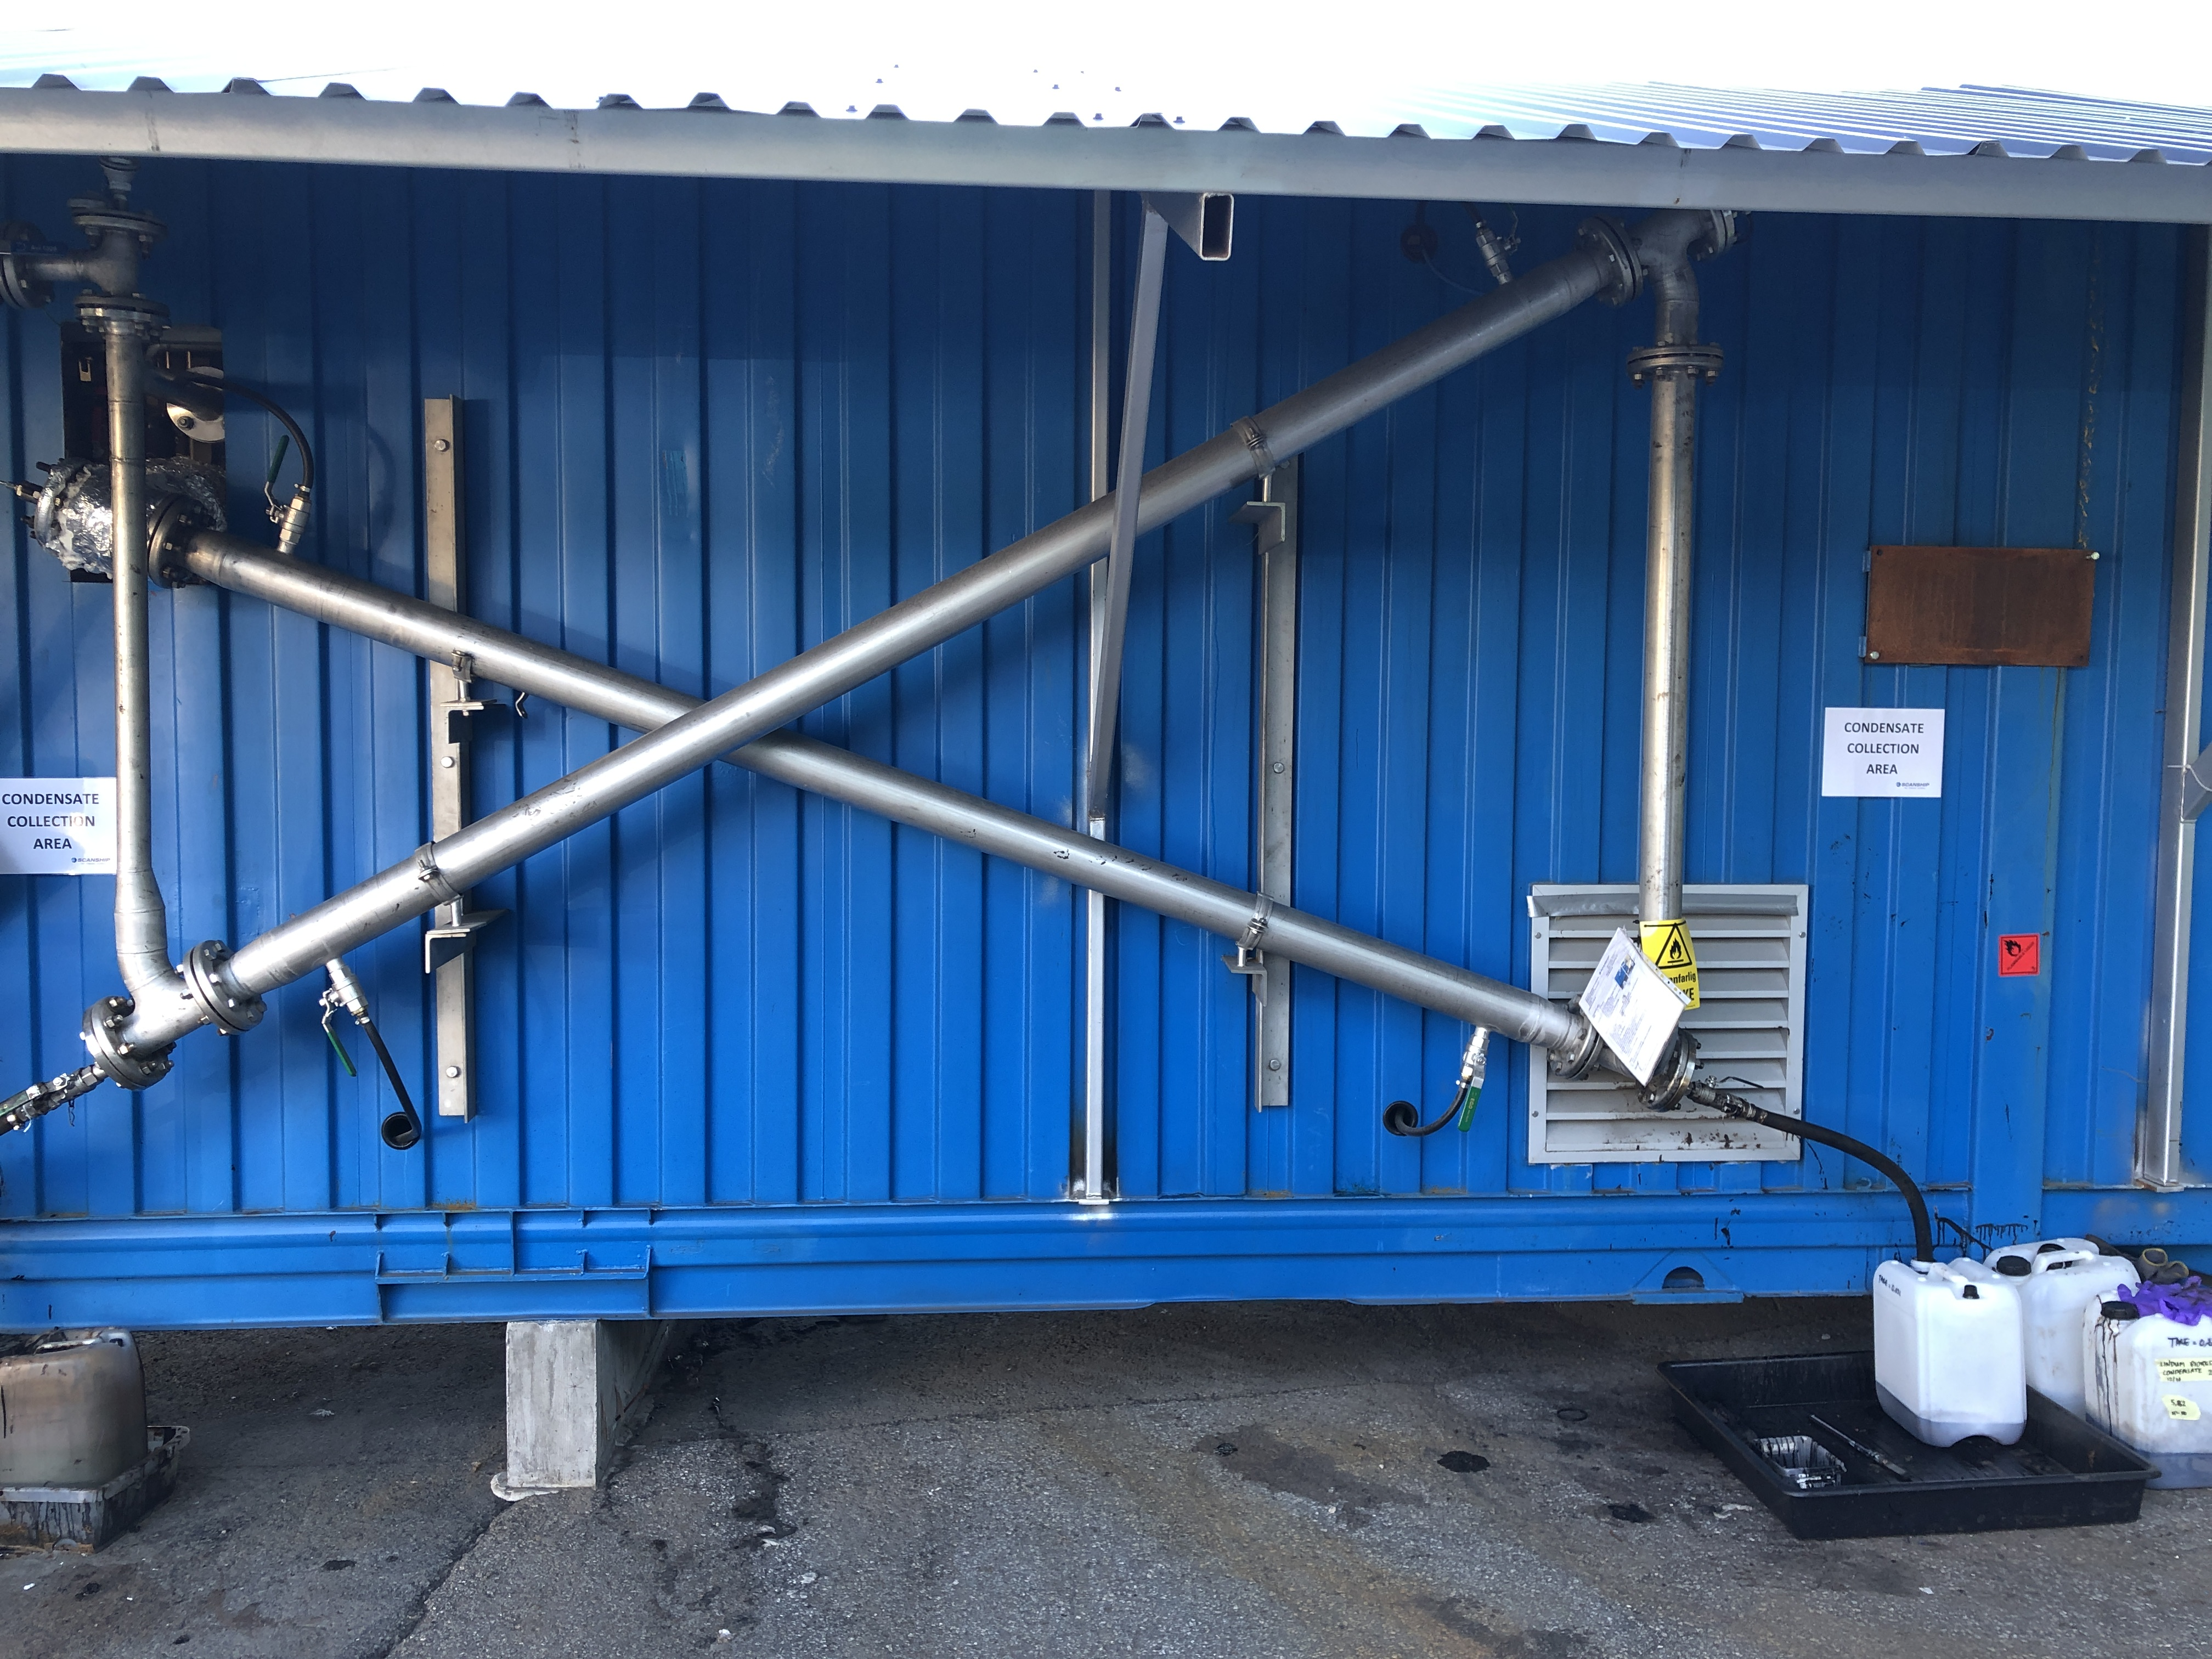
\includegraphics[width=0.74\linewidth,scale=0.74]{Bilder/Pyrolysis/Condenser.png}
    \caption{Syn-gas condenser.}
    \label{fig:condenser}
\end{figure}

\begin{figure}
    \centering
    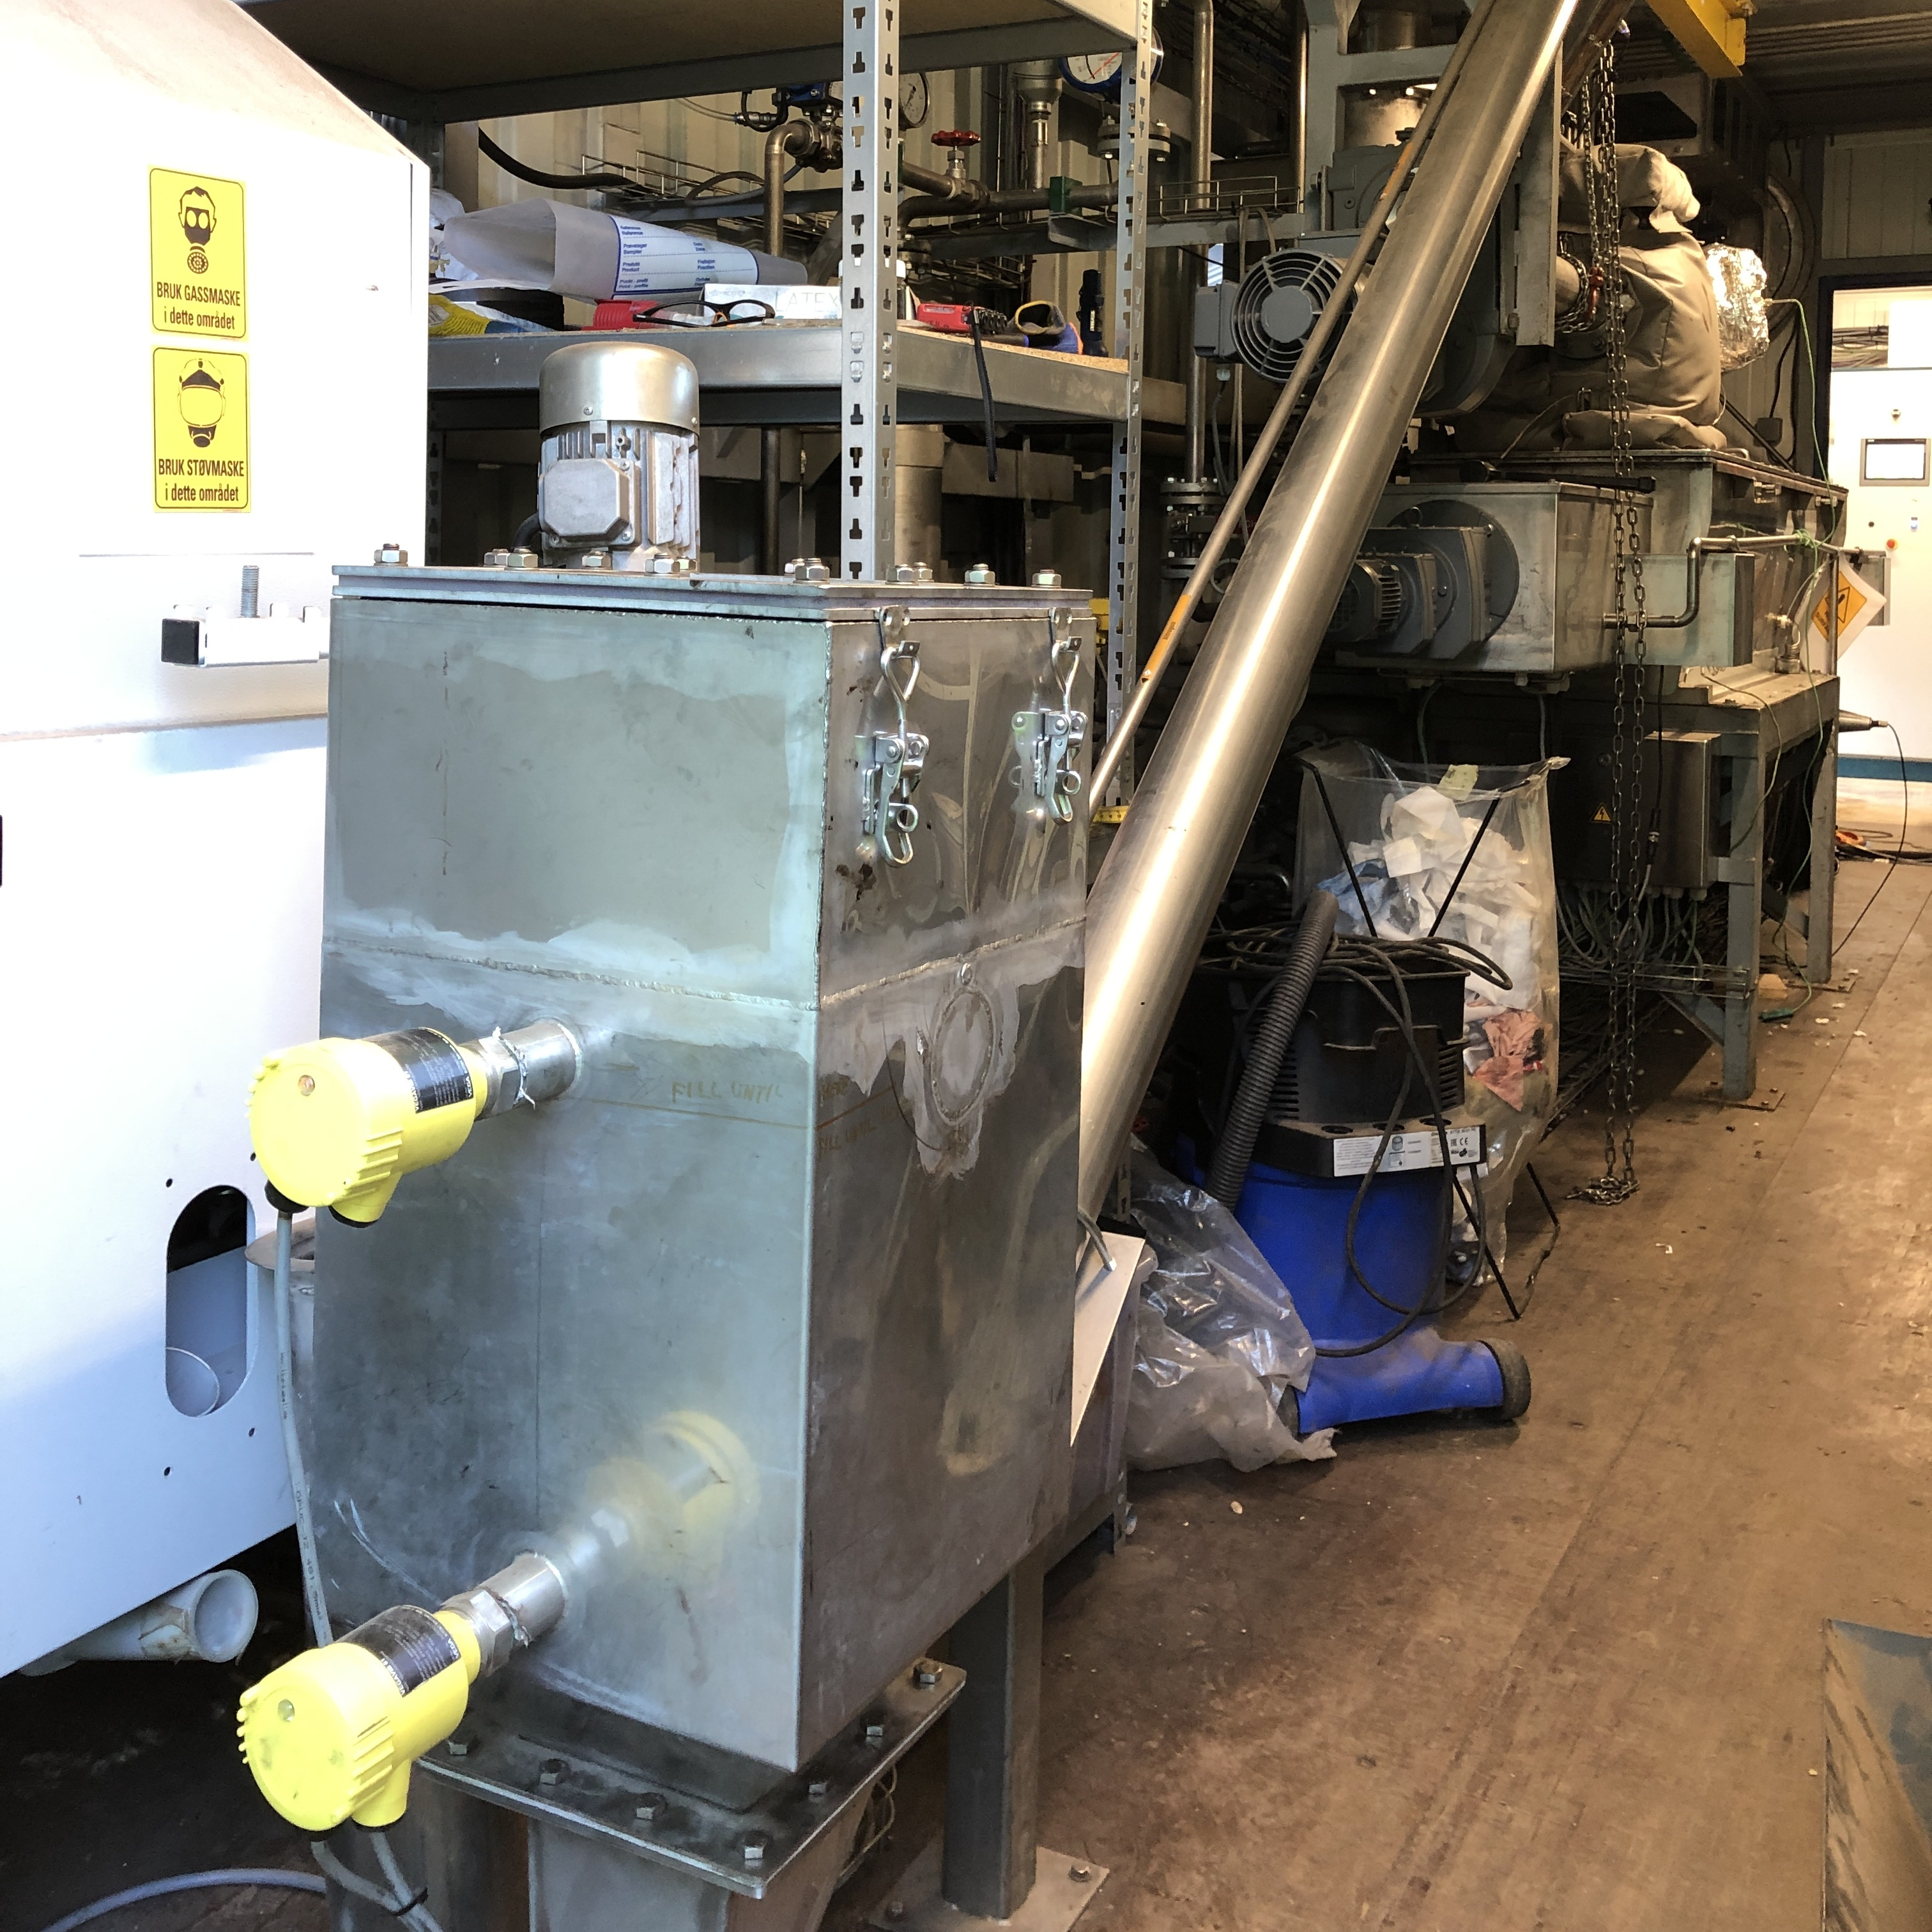
\includegraphics[width=0.6\linewidth,scale=0.6]{Bilder/Pyrolysis/Feeder.jpg}
    \caption{Starting point for the pyrolysis process where feedstock pellets are added to the system and transported with a rotating screw up the pipe on the photo that leads to the pyrolysis chamber.}
    \label{fig:feeder}
\end{figure}

\begin{figure}
    \centering
     \begin{subfigure}[t]{\linewidth}
         \centering
         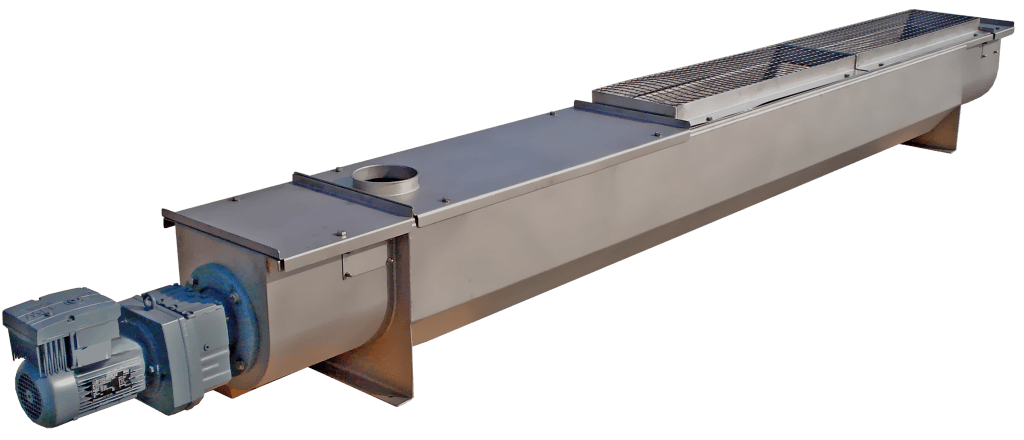
\includegraphics[width=0.74\linewidth,scale=0.74]{Bilder/Pyrolysis/PyrolyzerChamber.png}
         \caption{}
     \end{subfigure}
    \centering
    \begin{subfigure}[b]{\linewidth}
         \centering
         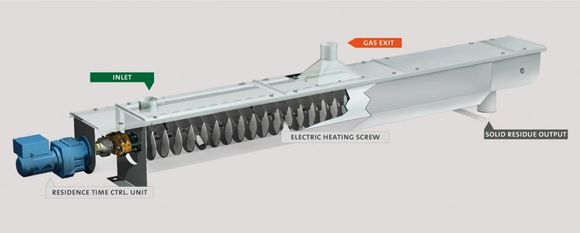
\includegraphics[width=0.74\linewidth,scale=0.74]{Bilder/Pyrolysis/spirajoule.jpeg}
         \caption{}
     \end{subfigure}
    \caption{\textbf{(a)} external view of the pyrolysis chamber, \textbf{(b)} internal view of the pyrolysis chamber. The Spirajoule\textsuperscript{\textregistered} is heated to the desired pyrolysis temperature and the speed of rotation is set to the wanted residence. Adopted from \url{https://www.biogreen-energy.com/spirajoule}.}
    \label{fig:pyrolysischamber}
\end{figure}

Been banned with new guidelines and regulations but there is still much left in the unsaturated zone heavily contaminated with PFAS (what are the concentrations of the various PFASs?) NGI document? Firefighting training site at Gardermoen, Norway used these substances since 1989. Ullensaker sludge


The batch tests were prepared with a liquid to solid mass ratio (L/S) of 500 for biochar and L/S of 10 for soil amended with 2\% biochar in accordance with CEN EN 12457 with modifications described in \citep{Hale2017fire, kupryianchyk2016biochar}. An overview of the experimental setup for the batch tests is given in \cref{fig:batchtests_flowchart} and an illustration of the batch test experiment procedure is in \cref{fig:batchtest_setup}. Finer details in the differences between each batch test category are given in the subsections below. 

All PP tubes were rinsed three times with 50\% MeOH prior to sample preparation to extract any potential PFAS contamination. The dry matter (biochar or biochar+soil) was added to pre-cleaned 50 mL PP centrifuge tubes and spiked with either individual PFCAs or a cocktail of all six PFCAs at the concentrations specified in \cref{tab:spikeConcentrations} to a final sample volume of 50 mL. The samples were assured to contain \textless 10\% MeOH, which is the upper limit for which methanol does not influence sorption \citep{arvaniti2014}. 

The batch tests were shaken end-over-end (9 rpm) and/or agitated on a shaking table (160 rpm) in room temperature (23\textdegree C) for at least 14 days to reach equilibrium \citep{higgins2006sorption}. The samples were then filtered through a 0.45 \textmu m Minisart\textsuperscript{\textregistered} regenerated cellulose syringe filter into PP tubes according to the methods described in \cite{Sorengard2019}. Loss of biochar to the walls of the syringe was quantified to maintain a full mass balance when analyzing the partitioning of PFCA between the solid and liquid phase and is in \cref{appSec:misclab}. Therefore, a 100\% mass balance was assumed when calculating partitioning between sorbent and water by subtracting the initial spike concentration from the measured filtrate concentration.  



\subsubsection{Biochar-water batch tests}
100$\pm$4 mg biochar was weighed for the biochar-water batch tests and placed into pre-cleaned 50 mL PP tubes. The tubes were filled half up of Milli-Q water. In each tube, stock PFCA was pipetted using micro- (5-50 $\mu$L and 200-1000 $\mu$L) and milli pipettes (2-10 mL) into the char-water solution to make 10 dilutions for each of the 6 PFCAs in even intervals within the concentration points in \cref{tab:spikeConcentrations}. Some tubes were added Milli-Q water up to the 50 mL mark and some samples were weighed after evaluating after some time that weighing would be more accurate and precise. The same ten concentrations were used to spike CWC, ULS and DSL batch tests. A cocktail batch test was prepared for the three biochars using the same relative amounts of each TC as the single-spike samples at SC10 (SC10-MIX), which was spiked directly into the sample tubes. The cumulative CMC (critical micelle concentration) for the six PFCA at SC10 was assured not to be an issue for the concentration range considered \citep{bhhatarai2011,ding2013physicochemical}.

\subsubsection{Soil-biochar-water batch tests}\label{sec:S-BC}
5\textpm 0.005 g soil and 0.1\textpm 0.0004 g biochar were weighed for each soil-BC-water batch test. A cocktail standard was prepared before spiking the samples using the same proportions at SC10 as for the biochar-water batch test. The difference between the two methods used to spike cocktail samples is a potential source of error for later comparison of sorption attenuation. and shaken in an end-over-end shaker for \textgreater 14 days. The batch tests were centrifuged to remove as many particles from suspension as possible. However, filtration still required frequent filter change due to clogging (up to three times per sample).

Matrix effects (MEs, \%) during measurements were assessed and estimated as X, X, X, X, X, X for PFPeA, PFHxA, PFHpA, PFOA, PFNA, and PFDA, respectively.

Langmuir dual-mode are other relations used to describe adsorption. This study uses the Freundlich relation to describe the equilibrium distribution of PFAS between biochar, soil and water. 

Langmuir assumes sorption sites are finite and adsorption is limited to monolayer coverage, a sorption maximum is reached, reversible process. Langmuir assumptions will not work in the presence of soil

Langmuir: assumes constant sorption free energy (ideal monolayer coverage, identical sites, no interaction between sorbates)
Freundlich: assumes log distribution of sorption free energies, more empiric, often better fit and comparison with literature

\citep{du2014adsorption}: Langmuir model usually describes the adsorption isotherms of PFOS and PFOA well, so need to explain why we chose Freundlich. Monolayer sorption is not realistic. 

"The Freundlich relation differs from that of Langmuir in that it does not consider all sites on the adsorbent surface to be equal but rather adsorption becomes progressively more difficult as more and more adsorbate accumulates. Furthermore, it is assumed that, once the surface is covered, additional adsorbed species can still be accommodated. In other words, multilayer adsorption is predicted by this relation" \citep{vanloon2017Ch14}
Limitation of the Freundlich model is that it does not predict an adsorption maximum. 
Freundlich relation is good for modeling the equilibrium distribution at low concentrations of the organic solute and small molecules \citep{vanloon2017Ch14}

Ullensaker is a municipality in Oslo that housed a firefighting training site at Gardermoen where PFAS added to aqueous film forming foam (AFFF) have been used since 1989 \citep{Hale2017fire}.

Sorption of PFAS to biochar is expected to follow the Freundlich sorption isotherm \citep{Hale2016, kupryianchyk2016biochar}. This Non-linearity implies that sorption becomes weaker at higher concentrations \cref{eq:Freundlich}. The Freundlich sorption isotherm is further discussed in \cref{sec:data_analysis}. 

This is according to the standard method for measuring pH in soil. It is common to add CaCl\textsubscript{2} if the soil has a low ionic strength, but this was, however, considered unnecessary in the presence of biochar since biochar contains a high amount of soluble ions. 